\documentclass[1p]{elsarticle_modified}
%\bibliographystyle{elsarticle-num}

%\usepackage[colorlinks]{hyperref}
%\usepackage{abbrmath_seonhwa} %\Abb, \Ascr, \Acal ,\Abf, \Afrak
\usepackage{amsfonts}
\usepackage{amssymb}
\usepackage{amsmath}
\usepackage{amsthm}
\usepackage{scalefnt}
\usepackage{amsbsy}
\usepackage{kotex}
\usepackage{caption}
\usepackage{subfig}
\usepackage{color}
\usepackage{graphicx}
\usepackage{xcolor} %% white, black, red, green, blue, cyan, magenta, yellow
\usepackage{float}
\usepackage{setspace}
\usepackage{hyperref}

\usepackage{tikz}
\usetikzlibrary{arrows}

\usepackage{multirow}
\usepackage{array} % fixed length table
\usepackage{hhline}

%%%%%%%%%%%%%%%%%%%%%
\makeatletter
\renewcommand*\env@matrix[1][\arraystretch]{%
	\edef\arraystretch{#1}%
	\hskip -\arraycolsep
	\let\@ifnextchar\new@ifnextchar
	\array{*\c@MaxMatrixCols c}}
\makeatother %https://tex.stackexchange.com/questions/14071/how-can-i-increase-the-line-spacing-in-a-matrix
%%%%%%%%%%%%%%%

\usepackage[normalem]{ulem}

\newcommand{\msout}[1]{\ifmmode\text{\sout{\ensuremath{#1}}}\else\sout{#1}\fi}
%SOURCE: \msout is \stkout macro in https://tex.stackexchange.com/questions/20609/strikeout-in-math-mode

\newcommand{\cancel}[1]{
	\ifmmode
	{\color{red}\msout{#1}}
	\else
	{\color{red}\sout{#1}}
	\fi
}

\newcommand{\add}[1]{
	{\color{blue}\uwave{#1}}
}

\newcommand{\replace}[2]{
	\ifmmode
	{\color{red}\msout{#1}}{\color{blue}\uwave{#2}}
	\else
	{\color{red}\sout{#1}}{\color{blue}\uwave{#2}}
	\fi
}

\newcommand{\Sol}{\mathcal{S}} %segment
\newcommand{\D}{D} %diagram
\newcommand{\A}{\mathcal{A}} %arc


%%%%%%%%%%%%%%%%%%%%%%%%%%%%%5 test

\def\sl{\operatorname{\textup{SL}}(2,\Cbb)}
\def\psl{\operatorname{\textup{PSL}}(2,\Cbb)}
\def\quan{\mkern 1mu \triangleright \mkern 1mu}

\theoremstyle{definition}
\newtheorem{thm}{Theorem}[section]
\newtheorem{prop}[thm]{Proposition}
\newtheorem{lem}[thm]{Lemma}
\newtheorem{ques}[thm]{Question}
\newtheorem{cor}[thm]{Corollary}
\newtheorem{defn}[thm]{Definition}
\newtheorem{exam}[thm]{Example}
\newtheorem{rmk}[thm]{Remark}
\newtheorem{alg}[thm]{Algorithm}

\newcommand{\I}{\sqrt{-1}}
\begin{document}

%\begin{frontmatter}
%
%\title{Boundary parabolic representations of knots up to 8 crossings}
%
%%% Group authors per affiliation:
%\author{Yunhi Cho} 
%\address{Department of Mathematics, University of Seoul, Seoul, Korea}
%\ead{yhcho@uos.ac.kr}
%
%
%\author{Seonhwa Kim} %\fnref{s_kim}}
%\address{Center for Geometry and Physics, Institute for Basic Science, Pohang, 37673, Korea}
%\ead{ryeona17@ibs.re.kr}
%
%\author{Hyuk Kim}
%\address{Department of Mathematical Sciences, Seoul National University, Seoul 08826, Korea}
%\ead{hyukkim@snu.ac.kr}
%
%\author{Seokbeom Yoon}
%\address{Department of Mathematical Sciences, Seoul National University, Seoul, 08826,  Korea}
%\ead{sbyoon15@snu.ac.kr}
%
%\begin{abstract}
%We find all boundary parabolic representation of knots up to 8 crossings.
%
%\end{abstract}
%\begin{keyword}
%    \MSC[2010] 57M25 
%\end{keyword}
%
%\end{frontmatter}

%\linenumbers
%\tableofcontents
%
\newcommand\colored[1]{\textcolor{white}{\rule[-0.35ex]{0.8em}{1.4ex}}\kern-0.8em\color{red} #1}%
%\newcommand\colored[1]{\textcolor{white}{ #1}\kern-2.17ex	\textcolor{white}{ #1}\kern-1.81ex	\textcolor{white}{ #1}\kern-2.15ex\color{red}#1	}

{\Large $\underline{12a_{1102}~(K12a_{1102})}$}

\setlength{\tabcolsep}{10pt}
\renewcommand{\arraystretch}{1.6}
\vspace{1cm}\begin{tabular}{m{100pt}>{\centering\arraybackslash}m{274pt}}
\multirow{5}{120pt}{
	\centering
	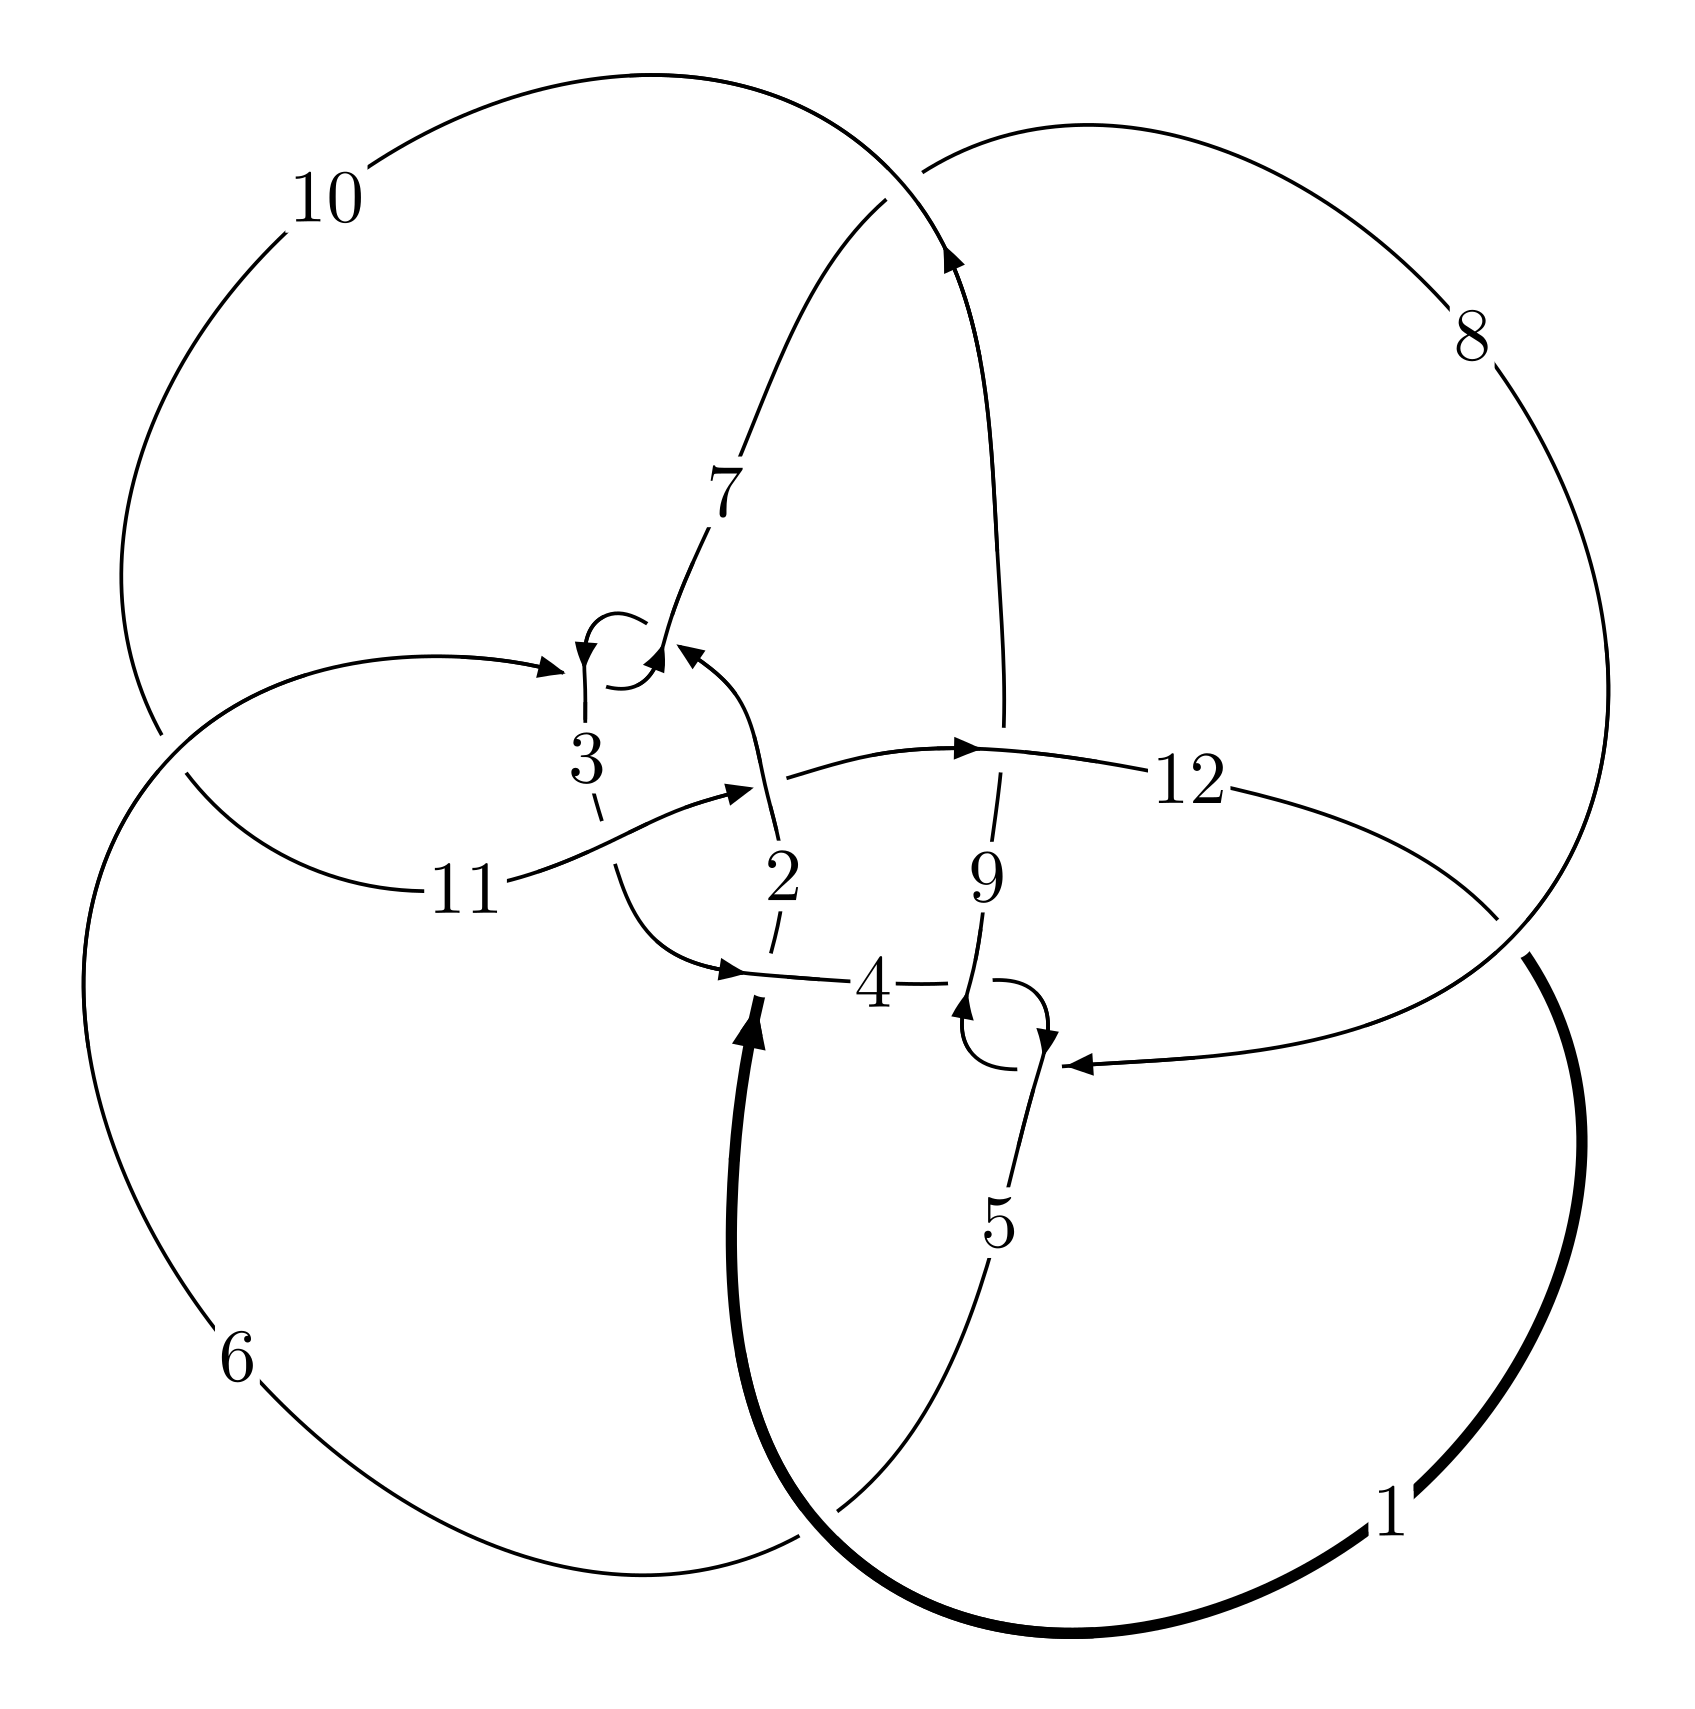
\includegraphics[width=112pt]{../../../GIT/diagram.site/Diagrams/png/1903_12a_1102.png}\\
\ \ \ A knot diagram\footnotemark}&
\allowdisplaybreaks
\textbf{Linearized knot diagam} \\
\cline{2-2}
 &
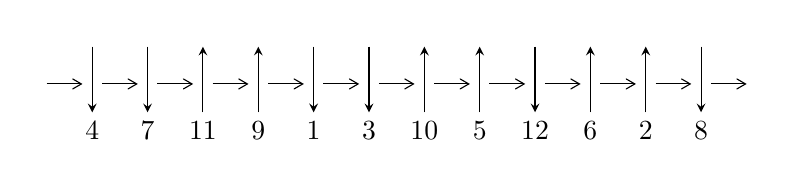
\begin{tikzpicture}[x=20pt, y=17pt]
	% nodes
	\node (C0) at (0, 0) {};
	\node (C1) at (1, 0) {};
	\node (C1U) at (1, +1) {};
	\node (C1D) at (1, -1) {4};

	\node (C2) at (2, 0) {};
	\node (C2U) at (2, +1) {};
	\node (C2D) at (2, -1) {7};

	\node (C3) at (3, 0) {};
	\node (C3U) at (3, +1) {};
	\node (C3D) at (3, -1) {11};

	\node (C4) at (4, 0) {};
	\node (C4U) at (4, +1) {};
	\node (C4D) at (4, -1) {9};

	\node (C5) at (5, 0) {};
	\node (C5U) at (5, +1) {};
	\node (C5D) at (5, -1) {1};

	\node (C6) at (6, 0) {};
	\node (C6U) at (6, +1) {};
	\node (C6D) at (6, -1) {3};

	\node (C7) at (7, 0) {};
	\node (C7U) at (7, +1) {};
	\node (C7D) at (7, -1) {10};

	\node (C8) at (8, 0) {};
	\node (C8U) at (8, +1) {};
	\node (C8D) at (8, -1) {5};

	\node (C9) at (9, 0) {};
	\node (C9U) at (9, +1) {};
	\node (C9D) at (9, -1) {12};

	\node (C10) at (10, 0) {};
	\node (C10U) at (10, +1) {};
	\node (C10D) at (10, -1) {6};

	\node (C11) at (11, 0) {};
	\node (C11U) at (11, +1) {};
	\node (C11D) at (11, -1) {2};

	\node (C12) at (12, 0) {};
	\node (C12U) at (12, +1) {};
	\node (C12D) at (12, -1) {8};
	\node (C13) at (13, 0) {};

	% arrows
	\draw[->,>={angle 60}]
	(C0) edge (C1) (C1) edge (C2) (C2) edge (C3) (C3) edge (C4) (C4) edge (C5) (C5) edge (C6) (C6) edge (C7) (C7) edge (C8) (C8) edge (C9) (C9) edge (C10) (C10) edge (C11) (C11) edge (C12) (C12) edge (C13) ;	\draw[->,>=stealth]
	(C1U) edge (C1D) (C2U) edge (C2D) (C3D) edge (C3U) (C4D) edge (C4U) (C5U) edge (C5D) (C6U) edge (C6D) (C7D) edge (C7U) (C8D) edge (C8U) (C9U) edge (C9D) (C10D) edge (C10U) (C11D) edge (C11U) (C12U) edge (C12D) ;
	\end{tikzpicture} \\
\hhline{~~} \\& 
\textbf{Solving Sequence} \\ \cline{2-2} 
 &
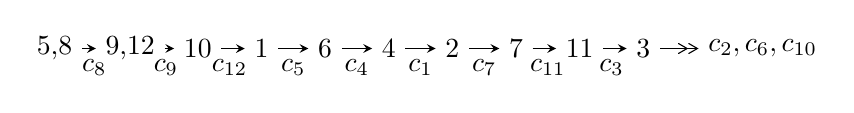
\begin{tikzpicture}[x=23pt, y=7pt]
	% node
	\node (A0) at (-1/8, 0) {5,8};
	\node (A1) at (17/16, 0) {9,12};
	\node (A2) at (17/8, 0) {10};
	\node (A3) at (25/8, 0) {1};
	\node (A4) at (33/8, 0) {6};
	\node (A5) at (41/8, 0) {4};
	\node (A6) at (49/8, 0) {2};
	\node (A7) at (57/8, 0) {7};
	\node (A8) at (65/8, 0) {11};
	\node (A9) at (73/8, 0) {3};
	\node (C1) at (1/2, -1) {$c_{8}$};
	\node (C2) at (13/8, -1) {$c_{9}$};
	\node (C3) at (21/8, -1) {$c_{12}$};
	\node (C4) at (29/8, -1) {$c_{5}$};
	\node (C5) at (37/8, -1) {$c_{4}$};
	\node (C6) at (45/8, -1) {$c_{1}$};
	\node (C7) at (53/8, -1) {$c_{7}$};
	\node (C8) at (61/8, -1) {$c_{11}$};
	\node (C9) at (69/8, -1) {$c_{3}$};
	\node (A10) at (11, 0) {$c_{2},c_{6},c_{10}$};

	% edge
	\draw[->,>=stealth]	
	(A0) edge (A1) (A1) edge (A2) (A2) edge (A3) (A3) edge (A4) (A4) edge (A5) (A5) edge (A6) (A6) edge (A7) (A7) edge (A8) (A8) edge (A9) ;
	\draw[->>,>={angle 60}]	
	(A9) edge (A10);
\end{tikzpicture} \\ 

\end{tabular} \\

\footnotetext{
The image of knot diagram is generated by the software ``\textbf{Draw programme}" developed by Andrew Bartholomew(\url{http://www.layer8.co.uk/maths/draw/index.htm\#Running-draw}), where we modified some parts for our purpose(\url{https://github.com/CATsTAILs/LinksPainter}).
}\phantom \\ \newline 
\centering \textbf{Ideals for irreducible components\footnotemark of $X_{\text{par}}$} 
 
\begin{align*}
I^u_{1}&=\langle 
3.67350\times10^{1261} u^{203}+1.84172\times10^{1262} u^{202}+\cdots+4.40006\times10^{1260} b+1.04500\times10^{1265},\\
\phantom{I^u_{1}}&\phantom{= \langle  }-4.46111\times10^{1264} u^{203}+4.52131\times10^{1265} u^{202}+\cdots+1.56246\times10^{1264} a+2.45131\times10^{1269},\\
\phantom{I^u_{1}}&\phantom{= \langle  }u^{204}+3 u^{203}+\cdots+4840 u+3551\rangle \\
I^u_{2}&=\langle 
-1.71279\times10^{68} u^{49}-6.40240\times10^{67} u^{48}+\cdots+2.21690\times10^{67} b+1.98493\times10^{69},\\
\phantom{I^u_{2}}&\phantom{= \langle  }-3.49182\times10^{66} u^{49}-3.83591\times10^{66} u^{48}+\cdots+1.30406\times10^{66} a+2.94979\times10^{67},\\
\phantom{I^u_{2}}&\phantom{= \langle  }u^{50}+3 u^{49}+\cdots+13 u+3\rangle \\
I^u_{3}&=\langle 
b+u,\;a+u,\;u^2- u+1\rangle \\
\\
\end{align*}
\raggedright * 3 irreducible components of $\dim_{\mathbb{C}}=0$, with total 256 representations.\\
\footnotetext{All coefficients of polynomials are rational numbers. But the coefficients are sometimes approximated in decimal forms when there is not enough margin.}
\newpage
\renewcommand{\arraystretch}{1}
\centering \section*{I. $I^u_{1}= \langle 3.67\times10^{1261} u^{203}+1.84\times10^{1262} u^{202}+\cdots+4.40\times10^{1260} b+1.04\times10^{1265},\;-4.46\times10^{1264} u^{203}+4.52\times10^{1265} u^{202}+\cdots+1.56\times10^{1264} a+2.45\times10^{1269},\;u^{204}+3 u^{203}+\cdots+4840 u+3551 \rangle$}
\flushleft \textbf{(i) Arc colorings}\\
\begin{tabular}{m{7pt} m{180pt} m{7pt} m{180pt} }
\flushright $a_{5}=$&$\begin{pmatrix}0\\u\end{pmatrix}$ \\
\flushright $a_{8}=$&$\begin{pmatrix}1\\0\end{pmatrix}$ \\
\flushright $a_{9}=$&$\begin{pmatrix}1\\- u^2\end{pmatrix}$ \\
\flushright $a_{12}=$&$\begin{pmatrix}2.85518 u^{203}-28.9371 u^{202}+\cdots-223331. u-156888.\\-8.34874 u^{203}-41.8568 u^{202}+\cdots-51131.0 u-23749.6\end{pmatrix}$ \\
\flushright $a_{10}=$&$\begin{pmatrix}50.8749 u^{203}+136.840 u^{202}+\cdots-27276.5 u-182971.\\7.65173 u^{203}+12.0064 u^{202}+\cdots-34318.5 u-54732.4\end{pmatrix}$ \\
\flushright $a_{1}=$&$\begin{pmatrix}11.2039 u^{203}+12.9197 u^{202}+\cdots-172200. u-133138.\\-8.34874 u^{203}-41.8568 u^{202}+\cdots-51131.0 u-23749.6\end{pmatrix}$ \\
\flushright $a_{6}=$&$\begin{pmatrix}-36.9992 u^{203}-133.745 u^{202}+\cdots-371456. u-68804.1\\-29.0147 u^{203}-81.8505 u^{202}+\cdots+18063.1 u+91150.3\end{pmatrix}$ \\
\flushright $a_{4}=$&$\begin{pmatrix}- u\\u^3+u\end{pmatrix}$ \\
\flushright $a_{2}=$&$\begin{pmatrix}12.2441 u^{203}-7.07902 u^{202}+\cdots-347730. u-234824.\\-0.719291 u^{203}-9.75512 u^{202}+\cdots+16196.1 u-4159.77\end{pmatrix}$ \\
\flushright $a_{7}=$&$\begin{pmatrix}13.7845 u^{203}+31.5172 u^{202}+\cdots-61495.8 u-114855.\\4.93226 u^{203}-15.2298 u^{202}+\cdots-370958. u-217639.\end{pmatrix}$ \\
\flushright $a_{11}=$&$\begin{pmatrix}35.9709 u^{203}+143.181 u^{202}+\cdots+533783. u+142600.\\-21.6892 u^{203}-79.6632 u^{202}+\cdots-122288. u-12547.3\end{pmatrix}$ \\
\flushright $a_{3}=$&$\begin{pmatrix}67.5293 u^{203}+213.644 u^{202}+\cdots+486394. u+5854.21\\24.6346 u^{203}+65.3690 u^{202}+\cdots+110435. u-46413.4\end{pmatrix}$\\&\end{tabular}
\flushleft \textbf{(ii) Obstruction class $= -1$}\\~\\
\flushleft \textbf{(iii) Cusp Shapes $= -265.682 u^{203}-624.980 u^{202}+\cdots+724985. u+1.44105\times10^{6}$}\\~\\
\newpage\renewcommand{\arraystretch}{1}
\flushleft \textbf{(iv) u-Polynomials at the component}\newline \\
\begin{tabular}{m{50pt}|m{274pt}}
Crossings & \hspace{64pt}u-Polynomials at each crossing \\
\hline $$\begin{aligned}c_{1}\end{aligned}$$&$\begin{aligned}
&4(4 u^{204}-110 u^{203}+\cdots-2861790 u+86273)
\end{aligned}$\\
\hline $$\begin{aligned}c_{2},c_{6}\end{aligned}$$&$\begin{aligned}
&u^{204}+3 u^{203}+\cdots+4840 u+3551
\end{aligned}$\\
\hline $$\begin{aligned}c_{3}\end{aligned}$$&$\begin{aligned}
&4(4 u^{204}-26 u^{203}+\cdots-4.51642\times10^{7} u+1.92815\times10^{7})
\end{aligned}$\\
\hline $$\begin{aligned}c_{4},c_{8}\end{aligned}$$&$\begin{aligned}
&u^{204}-3 u^{203}+\cdots-4840 u+3551
\end{aligned}$\\
\hline $$\begin{aligned}c_{5}\end{aligned}$$&$\begin{aligned}
&u^{204}+2 u^{203}+\cdots+3563896 u+160336
\end{aligned}$\\
\hline $$\begin{aligned}c_{7}\end{aligned}$$&$\begin{aligned}
&4(4 u^{204}+110 u^{203}+\cdots+2861790 u+86273)
\end{aligned}$\\
\hline $$\begin{aligned}c_{9}\end{aligned}$$&$\begin{aligned}
&u^{204}+10 u^{203}+\cdots+6000 u+2125
\end{aligned}$\\
\hline $$\begin{aligned}c_{10}\end{aligned}$$&$\begin{aligned}
&u^{204}-2 u^{203}+\cdots-3563896 u+160336
\end{aligned}$\\
\hline $$\begin{aligned}c_{11}\end{aligned}$$&$\begin{aligned}
&u^{204}-10 u^{203}+\cdots-6000 u+2125
\end{aligned}$\\
\hline $$\begin{aligned}c_{12}\end{aligned}$$&$\begin{aligned}
&4(4 u^{204}+26 u^{203}+\cdots+4.51642\times10^{7} u+1.92815\times10^{7})
\end{aligned}$\\
\hline
\end{tabular}\\~\\
\newpage\renewcommand{\arraystretch}{1}
\flushleft \textbf{(v) Riley Polynomials at the component}\newline \\
\begin{tabular}{m{50pt}|m{274pt}}
Crossings & \hspace{64pt}Riley Polynomials at each crossing \\
\hline $$\begin{aligned}c_{1},c_{7}\end{aligned}$$&$\begin{aligned}
&16(16 y^{204}-12 y^{203}+\cdots+4.27091\times10^{9} y+7.44303\times10^{9})
\end{aligned}$\\
\hline $$\begin{aligned}c_{2},c_{4},c_{6}\\c_{8}\end{aligned}$$&$\begin{aligned}
&y^{204}+131 y^{203}+\cdots+1159746294 y+12609601
\end{aligned}$\\
\hline $$\begin{aligned}c_{3},c_{12}\end{aligned}$$&$\begin{aligned}
&16\\
&\cdot(16 y^{204}-748 y^{203}+\cdots+42675043546023867 y+371776280813001)
\end{aligned}$\\
\hline $$\begin{aligned}c_{5},c_{10}\end{aligned}$$&$\begin{aligned}
&y^{204}-16 y^{203}+\cdots+2207655010624 y+25707632896
\end{aligned}$\\
\hline $$\begin{aligned}c_{9},c_{11}\end{aligned}$$&$\begin{aligned}
&y^{204}-46 y^{203}+\cdots+487217500 y+4515625
\end{aligned}$\\
\hline
\end{tabular}\\~\\
\newpage\flushleft \textbf{(vi) Complex Volumes and Cusp Shapes}
$$\begin{array}{c|c|c}  
\text{Solutions to }I^u_{1}& \I (\text{vol} + \sqrt{-1}CS) & \text{Cusp shape}\\
 \hline 
\begin{aligned}
u &= -0.051229 + 0.997299 I \\
a &= -1.95825 - 1.29139 I \\
b &= -0.780105 - 0.063644 I\end{aligned}
 & -3.51918 - 1.04221 I & \phantom{-0.000000 } 0 \\ \hline\begin{aligned}
u &= -0.051229 - 0.997299 I \\
a &= -1.95825 + 1.29139 I \\
b &= -0.780105 + 0.063644 I\end{aligned}
 & -3.51918 + 1.04221 I & \phantom{-0.000000 } 0 \\ \hline\begin{aligned}
u &= -0.054273 + 1.001330 I \\
a &= \phantom{-}0.779443 + 0.927451 I \\
b &= \phantom{-}0.650174 - 0.786115 I\end{aligned}
 & -3.56627 + 0.68723 I & \phantom{-0.000000 } 0 \\ \hline\begin{aligned}
u &= -0.054273 - 1.001330 I \\
a &= \phantom{-}0.779443 - 0.927451 I \\
b &= \phantom{-}0.650174 + 0.786115 I\end{aligned}
 & -3.56627 - 0.68723 I & \phantom{-0.000000 } 0 \\ \hline\begin{aligned}
u &= \phantom{-}0.212067 + 0.965336 I \\
a &= -0.968189 - 0.329212 I \\
b &= -0.625468 - 1.070670 I\end{aligned}
 & -1.17263 + 3.43391 I & \phantom{-0.000000 } 0 \\ \hline\begin{aligned}
u &= \phantom{-}0.212067 - 0.965336 I \\
a &= -0.968189 + 0.329212 I \\
b &= -0.625468 + 1.070670 I\end{aligned}
 & -1.17263 - 3.43391 I & \phantom{-0.000000 } 0 \\ \hline\begin{aligned}
u &= -0.401804 + 0.934446 I \\
a &= \phantom{-}0.381037 - 0.009674 I \\
b &= \phantom{-}0.274551 + 1.198520 I\end{aligned}
 & \phantom{-}2.37355 - 5.11261 I & \phantom{-0.000000 } 0 \\ \hline\begin{aligned}
u &= -0.401804 - 0.934446 I \\
a &= \phantom{-}0.381037 + 0.009674 I \\
b &= \phantom{-}0.274551 - 1.198520 I\end{aligned}
 & \phantom{-}2.37355 + 5.11261 I & \phantom{-0.000000 } 0 \\ \hline\begin{aligned}
u &= \phantom{-}0.148839 + 1.018130 I \\
a &= -2.62495 + 0.06301 I \\
b &= -1.75547 - 0.08177 I\end{aligned}
 & -0.97297 + 2.59722 I & \phantom{-0.000000 } 0 \\ \hline\begin{aligned}
u &= \phantom{-}0.148839 - 1.018130 I \\
a &= -2.62495 - 0.06301 I \\
b &= -1.75547 + 0.08177 I\end{aligned}
 & -0.97297 - 2.59722 I & \phantom{-0.000000 } 0\\
 \hline 
 \end{array}$$\newpage$$\begin{array}{c|c|c}  
\text{Solutions to }I^u_{1}& \I (\text{vol} + \sqrt{-1}CS) & \text{Cusp shape}\\
 \hline 
\begin{aligned}
u &= -0.011556 + 1.031150 I \\
a &= \phantom{-}1.49935 - 0.88126 I \\
b &= \phantom{-}0.929016 + 0.650830 I\end{aligned}
 & -1.58126 - 5.70438 I & \phantom{-0.000000 } 0 \\ \hline\begin{aligned}
u &= -0.011556 - 1.031150 I \\
a &= \phantom{-}1.49935 + 0.88126 I \\
b &= \phantom{-}0.929016 - 0.650830 I\end{aligned}
 & -1.58126 + 5.70438 I & \phantom{-0.000000 } 0 \\ \hline\begin{aligned}
u &= -0.187032 + 1.014480 I \\
a &= -2.58656 - 0.47173 I \\
b &= -1.47357 - 0.21915 I\end{aligned}
 & \phantom{-0.000000 } -4.08470 I & \phantom{-0.000000 } 0 \\ \hline\begin{aligned}
u &= -0.187032 - 1.014480 I \\
a &= -2.58656 + 0.47173 I \\
b &= -1.47357 + 0.21915 I\end{aligned}
 & \phantom{-0.000000 -}4.08470 I & \phantom{-0.000000 } 0 \\ \hline\begin{aligned}
u &= -0.459756 + 0.850378 I \\
a &= -0.515838 + 1.247530 I \\
b &= -1.169510 - 0.029616 I\end{aligned}
 & -0.58413 + 4.40088 I & \phantom{-0.000000 } 0 \\ \hline\begin{aligned}
u &= -0.459756 - 0.850378 I \\
a &= -0.515838 - 1.247530 I \\
b &= -1.169510 + 0.029616 I\end{aligned}
 & -0.58413 - 4.40088 I & \phantom{-0.000000 } 0 \\ \hline\begin{aligned}
u &= \phantom{-}0.211289 + 0.942603 I \\
a &= \phantom{-}0.013430 + 1.023340 I \\
b &= \phantom{-}0.55197 + 1.84637 I\end{aligned}
 & \phantom{-}4.37297 + 0.53308 I & \phantom{-0.000000 } 0 \\ \hline\begin{aligned}
u &= \phantom{-}0.211289 - 0.942603 I \\
a &= \phantom{-}0.013430 - 1.023340 I \\
b &= \phantom{-}0.55197 - 1.84637 I\end{aligned}
 & \phantom{-}4.37297 - 0.53308 I & \phantom{-0.000000 } 0 \\ \hline\begin{aligned}
u &= \phantom{-}0.307793 + 0.989208 I \\
a &= \phantom{-}0.13731 + 1.41503 I \\
b &= \phantom{-}0.58364 + 2.00724 I\end{aligned}
 & \phantom{-}2.62359 + 12.41050 I & \phantom{-0.000000 } 0 \\ \hline\begin{aligned}
u &= \phantom{-}0.307793 - 0.989208 I \\
a &= \phantom{-}0.13731 - 1.41503 I \\
b &= \phantom{-}0.58364 - 2.00724 I\end{aligned}
 & \phantom{-}2.62359 - 12.41050 I & \phantom{-0.000000 } 0\\
 \hline 
 \end{array}$$\newpage$$\begin{array}{c|c|c}  
\text{Solutions to }I^u_{1}& \I (\text{vol} + \sqrt{-1}CS) & \text{Cusp shape}\\
 \hline 
\begin{aligned}
u &= -0.746233 + 0.723442 I \\
a &= \phantom{-}0.836172 - 0.797491 I \\
b &= \phantom{-}0.967089 - 0.556374 I\end{aligned}
 & \phantom{-}3.95477 + 3.85138 I & \phantom{-0.000000 } 0 \\ \hline\begin{aligned}
u &= -0.746233 - 0.723442 I \\
a &= \phantom{-}0.836172 + 0.797491 I \\
b &= \phantom{-}0.967089 + 0.556374 I\end{aligned}
 & \phantom{-}3.95477 - 3.85138 I & \phantom{-0.000000 } 0 \\ \hline\begin{aligned}
u &= \phantom{-}0.226179 + 0.932604 I \\
a &= \phantom{-}3.12258 - 0.52225 I \\
b &= \phantom{-}0.411370 - 0.470927 I\end{aligned}
 & \phantom{-}2.66918 + 11.39430 I & \phantom{-0.000000 } 0 \\ \hline\begin{aligned}
u &= \phantom{-}0.226179 - 0.932604 I \\
a &= \phantom{-}3.12258 + 0.52225 I \\
b &= \phantom{-}0.411370 + 0.470927 I\end{aligned}
 & \phantom{-}2.66918 - 11.39430 I & \phantom{-0.000000 } 0 \\ \hline\begin{aligned}
u &= \phantom{-}0.950146 + 0.099052 I \\
a &= \phantom{-}0.110065 + 0.108369 I \\
b &= \phantom{-}0.920127 + 0.718542 I\end{aligned}
 & -0.33838 - 4.08024 I & \phantom{-0.000000 } 0 \\ \hline\begin{aligned}
u &= \phantom{-}0.950146 - 0.099052 I \\
a &= \phantom{-}0.110065 - 0.108369 I \\
b &= \phantom{-}0.920127 - 0.718542 I\end{aligned}
 & -0.33838 + 4.08024 I & \phantom{-0.000000 } 0 \\ \hline\begin{aligned}
u &= -0.268180 + 1.010710 I \\
a &= \phantom{-}0.16343 - 1.43207 I \\
b &= \phantom{-}0.66592 - 1.98156 I\end{aligned}
 & -1.40036 - 6.34486 I & \phantom{-0.000000 } 0 \\ \hline\begin{aligned}
u &= -0.268180 - 1.010710 I \\
a &= \phantom{-}0.16343 + 1.43207 I \\
b &= \phantom{-}0.66592 + 1.98156 I\end{aligned}
 & -1.40036 + 6.34486 I & \phantom{-0.000000 } 0 \\ \hline\begin{aligned}
u &= -0.829479 + 0.462983 I \\
a &= -0.166613 - 0.610878 I \\
b &= \phantom{-}1.18333 - 0.84935 I\end{aligned}
 & \phantom{-}3.23806 + 5.58875 I & \phantom{-0.000000 } 0 \\ \hline\begin{aligned}
u &= -0.829479 - 0.462983 I \\
a &= -0.166613 + 0.610878 I \\
b &= \phantom{-}1.18333 + 0.84935 I\end{aligned}
 & \phantom{-}3.23806 - 5.58875 I & \phantom{-0.000000 } 0\\
 \hline 
 \end{array}$$\newpage$$\begin{array}{c|c|c}  
\text{Solutions to }I^u_{1}& \I (\text{vol} + \sqrt{-1}CS) & \text{Cusp shape}\\
 \hline 
\begin{aligned}
u &= \phantom{-}0.939682 + 0.095860 I \\
a &= -0.337457 + 0.268608 I \\
b &= -0.424168 - 0.795765 I\end{aligned}
 & \phantom{-}5.93767 - 3.95269 I & \phantom{-0.000000 } 0 \\ \hline\begin{aligned}
u &= \phantom{-}0.939682 - 0.095860 I \\
a &= -0.337457 - 0.268608 I \\
b &= -0.424168 + 0.795765 I\end{aligned}
 & \phantom{-}5.93767 + 3.95269 I & \phantom{-0.000000 } 0 \\ \hline\begin{aligned}
u &= \phantom{-}0.695440 + 0.796725 I \\
a &= \phantom{-}0.266504 - 0.702020 I \\
b &= -0.481935 + 0.457813 I\end{aligned}
 & -1.26449 + 1.30166 I & \phantom{-0.000000 } 0 \\ \hline\begin{aligned}
u &= \phantom{-}0.695440 - 0.796725 I \\
a &= \phantom{-}0.266504 + 0.702020 I \\
b &= -0.481935 - 0.457813 I\end{aligned}
 & -1.26449 - 1.30166 I & \phantom{-0.000000 } 0 \\ \hline\begin{aligned}
u &= -0.833528 + 0.432817 I \\
a &= \phantom{-}0.348893 + 0.168592 I \\
b &= -0.686112 - 0.669672 I\end{aligned}
 & \phantom{-}1.95629 - 8.25786 I & \phantom{-0.000000 } 0 \\ \hline\begin{aligned}
u &= -0.833528 - 0.432817 I \\
a &= \phantom{-}0.348893 - 0.168592 I \\
b &= -0.686112 + 0.669672 I\end{aligned}
 & \phantom{-}1.95629 + 8.25786 I & \phantom{-0.000000 } 0 \\ \hline\begin{aligned}
u &= \phantom{-}0.801995 + 0.482457 I \\
a &= \phantom{-}0.819543 - 0.367997 I \\
b &= -0.349244 - 0.796838 I\end{aligned}
 & \phantom{-}3.56627 - 0.68723 I & \phantom{-0.000000 } 0 \\ \hline\begin{aligned}
u &= \phantom{-}0.801995 - 0.482457 I \\
a &= \phantom{-}0.819543 + 0.367997 I \\
b &= -0.349244 + 0.796838 I\end{aligned}
 & \phantom{-}3.56627 + 0.68723 I & \phantom{-0.000000 } 0 \\ \hline\begin{aligned}
u &= -1.052890 + 0.171869 I \\
a &= \phantom{-}0.167718 + 0.136237 I \\
b &= -0.881069 + 0.730076 I\end{aligned}
 & \phantom{-}5.51079 + 4.29685 I & \phantom{-0.000000 } 0 \\ \hline\begin{aligned}
u &= -1.052890 - 0.171869 I \\
a &= \phantom{-}0.167718 - 0.136237 I \\
b &= -0.881069 - 0.730076 I\end{aligned}
 & \phantom{-}5.51079 - 4.29685 I & \phantom{-0.000000 } 0\\
 \hline 
 \end{array}$$\newpage$$\begin{array}{c|c|c}  
\text{Solutions to }I^u_{1}& \I (\text{vol} + \sqrt{-1}CS) & \text{Cusp shape}\\
 \hline 
\begin{aligned}
u &= -1.027960 + 0.287527 I \\
a &= -0.0552375 - 0.0154616 I \\
b &= -0.402642 + 0.588854 I\end{aligned}
 & \phantom{-}3.12986 - 1.22046 I & \phantom{-0.000000 } 0 \\ \hline\begin{aligned}
u &= -1.027960 - 0.287527 I \\
a &= -0.0552375 + 0.0154616 I \\
b &= -0.402642 - 0.588854 I\end{aligned}
 & \phantom{-}3.12986 + 1.22046 I & \phantom{-0.000000 } 0 \\ \hline\begin{aligned}
u &= -0.434269 + 0.993849 I \\
a &= -1.010430 - 0.622410 I \\
b &= \phantom{-}0.0229985 + 0.1125580 I\end{aligned}
 & \phantom{-}3.24228 - 6.46386 I & \phantom{-0.000000 } 0 \\ \hline\begin{aligned}
u &= -0.434269 - 0.993849 I \\
a &= -1.010430 + 0.622410 I \\
b &= \phantom{-}0.0229985 - 0.1125580 I\end{aligned}
 & \phantom{-}3.24228 + 6.46386 I & \phantom{-0.000000 } 0 \\ \hline\begin{aligned}
u &= \phantom{-}0.902975 + 0.041911 I \\
a &= \phantom{-}0.222078 + 0.022680 I \\
b &= \phantom{-}0.901835 - 0.742438 I\end{aligned}
 & -0.36015 + 4.15367 I & \phantom{-0.000000 } 0 \\ \hline\begin{aligned}
u &= \phantom{-}0.902975 - 0.041911 I \\
a &= \phantom{-}0.222078 - 0.022680 I \\
b &= \phantom{-}0.901835 + 0.742438 I\end{aligned}
 & -0.36015 - 4.15367 I & \phantom{-0.000000 } 0 \\ \hline\begin{aligned}
u &= -0.198646 + 0.863874 I \\
a &= \phantom{-}3.19678 - 0.09619 I \\
b &= \phantom{-}0.268321 + 0.498301 I\end{aligned}
 & -0.34975 - 5.08554 I & \phantom{-0.000000 } 0 \\ \hline\begin{aligned}
u &= -0.198646 - 0.863874 I \\
a &= \phantom{-}3.19678 + 0.09619 I \\
b &= \phantom{-}0.268321 - 0.498301 I\end{aligned}
 & -0.34975 + 5.08554 I & \phantom{-0.000000 } 0 \\ \hline\begin{aligned}
u &= \phantom{-}0.125761 + 1.107940 I \\
a &= -1.57308 + 0.88124 I \\
b &= -0.766669 - 0.031549 I\end{aligned}
 & -2.37355 + 5.11261 I & \phantom{-0.000000 } 0 \\ \hline\begin{aligned}
u &= \phantom{-}0.125761 - 1.107940 I \\
a &= -1.57308 - 0.88124 I \\
b &= -0.766669 + 0.031549 I\end{aligned}
 & -2.37355 - 5.11261 I & \phantom{-0.000000 } 0\\
 \hline 
 \end{array}$$\newpage$$\begin{array}{c|c|c}  
\text{Solutions to }I^u_{1}& \I (\text{vol} + \sqrt{-1}CS) & \text{Cusp shape}\\
 \hline 
\begin{aligned}
u &= \phantom{-}0.406129 + 0.780005 I \\
a &= \phantom{-}1.77929 - 0.56271 I \\
b &= \phantom{-}0.17390 - 1.68668 I\end{aligned}
 & \phantom{-}6.09283 + 1.75066 I & \phantom{-0.000000 } 0 \\ \hline\begin{aligned}
u &= \phantom{-}0.406129 - 0.780005 I \\
a &= \phantom{-}1.77929 + 0.56271 I \\
b &= \phantom{-}0.17390 + 1.68668 I\end{aligned}
 & \phantom{-}6.09283 - 1.75066 I & \phantom{-0.000000 } 0 \\ \hline\begin{aligned}
u &= \phantom{-}0.262782 + 0.838291 I \\
a &= -2.27900 + 1.10877 I \\
b &= -0.44587 + 1.90754 I\end{aligned}
 & \phantom{-}5.17607 + 1.25050 I & \phantom{-0.000000 } 0 \\ \hline\begin{aligned}
u &= \phantom{-}0.262782 - 0.838291 I \\
a &= -2.27900 - 1.10877 I \\
b &= -0.44587 - 1.90754 I\end{aligned}
 & \phantom{-}5.17607 - 1.25050 I & \phantom{-0.000000 } 0 \\ \hline\begin{aligned}
u &= \phantom{-}1.113650 + 0.135671 I \\
a &= -0.0212920 - 0.0847913 I \\
b &= -0.971497 - 0.742864 I\end{aligned}
 & \phantom{-0.000000 } -9.69632 I & \phantom{-0.000000 } 0 \\ \hline\begin{aligned}
u &= \phantom{-}1.113650 - 0.135671 I \\
a &= -0.0212920 + 0.0847913 I \\
b &= -0.971497 + 0.742864 I\end{aligned}
 & \phantom{-0.000000 -}9.69632 I & \phantom{-0.000000 } 0 \\ \hline\begin{aligned}
u &= \phantom{-}0.341590 + 0.803796 I \\
a &= \phantom{-}2.20474 - 0.13978 I \\
b &= \phantom{-}0.346484 - 0.722096 I\end{aligned}
 & \phantom{-}5.80970 + 0.97005 I & \phantom{-0.000000 } 0 \\ \hline\begin{aligned}
u &= \phantom{-}0.341590 - 0.803796 I \\
a &= \phantom{-}2.20474 + 0.13978 I \\
b &= \phantom{-}0.346484 + 0.722096 I\end{aligned}
 & \phantom{-}5.80970 - 0.97005 I & \phantom{-0.000000 } 0 \\ \hline\begin{aligned}
u &= -0.646136 + 0.562458 I \\
a &= \phantom{-}1.243000 + 0.275490 I \\
b &= -0.077992 + 0.704835 I\end{aligned}
 & \phantom{-}3.51918 + 1.04221 I & \phantom{-0.000000 } 0 \\ \hline\begin{aligned}
u &= -0.646136 - 0.562458 I \\
a &= \phantom{-}1.243000 - 0.275490 I \\
b &= -0.077992 - 0.704835 I\end{aligned}
 & \phantom{-}3.51918 - 1.04221 I & \phantom{-0.000000 } 0\\
 \hline 
 \end{array}$$\newpage$$\begin{array}{c|c|c}  
\text{Solutions to }I^u_{1}& \I (\text{vol} + \sqrt{-1}CS) & \text{Cusp shape}\\
 \hline 
\begin{aligned}
u &= \phantom{-}1.100020 + 0.337987 I \\
a &= \phantom{-}0.227969 + 0.305234 I \\
b &= \phantom{-}1.089140 + 0.512097 I\end{aligned}
 & \phantom{-}0.34975 - 5.08554 I & \phantom{-0.000000 } 0 \\ \hline\begin{aligned}
u &= \phantom{-}1.100020 - 0.337987 I \\
a &= \phantom{-}0.227969 - 0.305234 I \\
b &= \phantom{-}1.089140 - 0.512097 I\end{aligned}
 & \phantom{-}0.34975 + 5.08554 I & \phantom{-0.000000 } 0 \\ \hline\begin{aligned}
u &= -1.146350 + 0.147011 I \\
a &= -0.083504 + 0.157855 I \\
b &= -0.992856 + 0.777619 I\end{aligned}
 & \phantom{-}3.7066 + 15.6856 I & \phantom{-0.000000 } 0 \\ \hline\begin{aligned}
u &= -1.146350 - 0.147011 I \\
a &= -0.083504 - 0.157855 I \\
b &= -0.992856 - 0.777619 I\end{aligned}
 & \phantom{-}3.7066 - 15.6856 I & \phantom{-0.000000 } 0 \\ \hline\begin{aligned}
u &= -0.577482 + 0.614932 I \\
a &= -1.63594 + 0.97333 I \\
b &= -1.267250 - 0.087270 I\end{aligned}
 & \phantom{-}4.13767 - 8.80378 I & \phantom{-0.000000 } 0 \\ \hline\begin{aligned}
u &= -0.577482 - 0.614932 I \\
a &= -1.63594 - 0.97333 I \\
b &= -1.267250 + 0.087270 I\end{aligned}
 & \phantom{-}4.13767 + 8.80378 I & \phantom{-0.000000 } 0 \\ \hline\begin{aligned}
u &= -1.177070 + 0.065224 I \\
a &= \phantom{-}0.176090 - 0.259745 I \\
b &= \phantom{-}0.764803 - 0.725898 I\end{aligned}
 & \phantom{-}1.40036 + 6.34486 I & \phantom{-0.000000 } 0 \\ \hline\begin{aligned}
u &= -1.177070 - 0.065224 I \\
a &= \phantom{-}0.176090 + 0.259745 I \\
b &= \phantom{-}0.764803 + 0.725898 I\end{aligned}
 & \phantom{-}1.40036 - 6.34486 I & \phantom{-0.000000 } 0 \\ \hline\begin{aligned}
u &= \phantom{-}0.460944 + 1.085140 I \\
a &= -0.695550 - 0.967192 I \\
b &= -0.911272 - 0.058061 I\end{aligned}
 & -4.15789 - 0.07680 I & \phantom{-0.000000 } 0 \\ \hline\begin{aligned}
u &= \phantom{-}0.460944 - 1.085140 I \\
a &= -0.695550 + 0.967192 I \\
b &= -0.911272 + 0.058061 I\end{aligned}
 & -4.15789 + 0.07680 I & \phantom{-0.000000 } 0\\
 \hline 
 \end{array}$$\newpage$$\begin{array}{c|c|c}  
\text{Solutions to }I^u_{1}& \I (\text{vol} + \sqrt{-1}CS) & \text{Cusp shape}\\
 \hline 
\begin{aligned}
u &= -0.430137 + 1.103930 I \\
a &= \phantom{-}1.009960 - 0.761489 I \\
b &= \phantom{-}1.253360 - 0.644602 I\end{aligned}
 & \phantom{-}1.13472 - 3.92428 I & \phantom{-0.000000 } 0 \\ \hline\begin{aligned}
u &= -0.430137 - 1.103930 I \\
a &= \phantom{-}1.009960 + 0.761489 I \\
b &= \phantom{-}1.253360 + 0.644602 I\end{aligned}
 & \phantom{-}1.13472 + 3.92428 I & \phantom{-0.000000 } 0 \\ \hline\begin{aligned}
u &= \phantom{-}0.812439 + 0.049180 I \\
a &= \phantom{-}0.277213 + 0.853767 I \\
b &= \phantom{-}0.759008 + 0.392331 I\end{aligned}
 & \phantom{-}0.65302 - 2.35043 I & \phantom{-0.000000 } 0 \\ \hline\begin{aligned}
u &= \phantom{-}0.812439 - 0.049180 I \\
a &= \phantom{-}0.277213 - 0.853767 I \\
b &= \phantom{-}0.759008 - 0.392331 I\end{aligned}
 & \phantom{-}0.65302 + 2.35043 I & \phantom{-0.000000 } 0 \\ \hline\begin{aligned}
u &= \phantom{-}0.179935 + 0.791252 I \\
a &= -2.79268 + 0.98444 I \\
b &= -1.04510 + 1.05675 I\end{aligned}
 & \phantom{-}4.91227 + 1.46033 I & \phantom{-0.000000 } 0 \\ \hline\begin{aligned}
u &= \phantom{-}0.179935 - 0.791252 I \\
a &= -2.79268 - 0.98444 I \\
b &= -1.04510 - 1.05675 I\end{aligned}
 & \phantom{-}4.91227 - 1.46033 I & \phantom{-0.000000 } 0 \\ \hline\begin{aligned}
u &= \phantom{-}0.211600 + 1.171730 I \\
a &= \phantom{-}1.22377 + 1.59322 I \\
b &= \phantom{-}0.491009 - 0.349867 I\end{aligned}
 & -3.23806 + 5.58875 I & \phantom{-0.000000 } 0 \\ \hline\begin{aligned}
u &= \phantom{-}0.211600 - 1.171730 I \\
a &= \phantom{-}1.22377 - 1.59322 I \\
b &= \phantom{-}0.491009 + 0.349867 I\end{aligned}
 & -3.23806 - 5.58875 I & \phantom{-0.000000 } 0 \\ \hline\begin{aligned}
u &= -0.318190 + 0.736951 I \\
a &= \phantom{-}0.683196 - 1.069640 I \\
b &= -0.225095 + 1.023770 I\end{aligned}
 & -0.21738 + 2.51186 I & \phantom{-0.000000 } 0 \\ \hline\begin{aligned}
u &= -0.318190 - 0.736951 I \\
a &= \phantom{-}0.683196 + 1.069640 I \\
b &= -0.225095 - 1.023770 I\end{aligned}
 & -0.21738 - 2.51186 I & \phantom{-0.000000 } 0\\
 \hline 
 \end{array}$$\newpage$$\begin{array}{c|c|c}  
\text{Solutions to }I^u_{1}& \I (\text{vol} + \sqrt{-1}CS) & \text{Cusp shape}\\
 \hline 
\begin{aligned}
u &= \phantom{-}0.358100 + 0.711020 I \\
a &= \phantom{-}0.674272 + 0.287348 I \\
b &= -0.075062 - 1.247790 I\end{aligned}
 & \phantom{-}6.04666 + 2.26274 I & \phantom{-0.000000 } 0 \\ \hline\begin{aligned}
u &= \phantom{-}0.358100 - 0.711020 I \\
a &= \phantom{-}0.674272 - 0.287348 I \\
b &= -0.075062 + 1.247790 I\end{aligned}
 & \phantom{-}6.04666 - 2.26274 I & \phantom{-0.000000 } 0 \\ \hline\begin{aligned}
u &= \phantom{-}0.783654 + 0.135648 I \\
a &= \phantom{-}0.465779 - 0.221697 I \\
b &= -0.866825 + 0.444846 I\end{aligned}
 & -3.12986 + 1.22046 I & \phantom{-0.000000 } 0 \\ \hline\begin{aligned}
u &= \phantom{-}0.783654 - 0.135648 I \\
a &= \phantom{-}0.465779 + 0.221697 I \\
b &= -0.866825 - 0.444846 I\end{aligned}
 & -3.12986 - 1.22046 I & \phantom{-0.000000 } 0 \\ \hline\begin{aligned}
u &= -0.316560 + 1.166380 I \\
a &= -1.83827 + 0.18130 I \\
b &= -0.939328 - 1.026530 I\end{aligned}
 & -3.95477 - 3.85138 I & \phantom{-0.000000 } 0 \\ \hline\begin{aligned}
u &= -0.316560 - 1.166380 I \\
a &= -1.83827 - 0.18130 I \\
b &= -0.939328 + 1.026530 I\end{aligned}
 & -3.95477 + 3.85138 I & \phantom{-0.000000 } 0 \\ \hline\begin{aligned}
u &= -0.085483 + 0.784159 I \\
a &= \phantom{-}1.49002 - 0.55040 I \\
b &= \phantom{-}1.40094 - 1.20346 I\end{aligned}
 & \phantom{-}0.97297 + 2.59722 I & \phantom{-0.000000 } 0 \\ \hline\begin{aligned}
u &= -0.085483 - 0.784159 I \\
a &= \phantom{-}1.49002 + 0.55040 I \\
b &= \phantom{-}1.40094 + 1.20346 I\end{aligned}
 & \phantom{-}0.97297 - 2.59722 I & \phantom{-0.000000 } 0 \\ \hline\begin{aligned}
u &= \phantom{-}0.215596 + 0.755293 I \\
a &= -1.98259 + 0.19130 I \\
b &= \phantom{-}0.096965 - 0.433266 I\end{aligned}
 & -0.65302 + 2.35043 I & \phantom{-0.000000 } 0 \\ \hline\begin{aligned}
u &= \phantom{-}0.215596 - 0.755293 I \\
a &= -1.98259 - 0.19130 I \\
b &= \phantom{-}0.096965 + 0.433266 I\end{aligned}
 & -0.65302 - 2.35043 I & \phantom{-0.000000 } 0\\
 \hline 
 \end{array}$$\newpage$$\begin{array}{c|c|c}  
\text{Solutions to }I^u_{1}& \I (\text{vol} + \sqrt{-1}CS) & \text{Cusp shape}\\
 \hline 
\begin{aligned}
u &= -1.192830 + 0.260298 I \\
a &= \phantom{-}0.204097 - 0.131393 I \\
b &= \phantom{-}0.878574 - 0.352144 I\end{aligned}
 & \phantom{-}0.21738 + 2.51186 I & \phantom{-0.000000 } 0 \\ \hline\begin{aligned}
u &= -1.192830 - 0.260298 I \\
a &= \phantom{-}0.204097 + 0.131393 I \\
b &= \phantom{-}0.878574 + 0.352144 I\end{aligned}
 & \phantom{-}0.21738 - 2.51186 I & \phantom{-0.000000 } 0 \\ \hline\begin{aligned}
u &= \phantom{-}0.533930 + 1.105390 I \\
a &= \phantom{-}1.040090 + 0.112544 I \\
b &= \phantom{-}0.856992 - 1.081250 I\end{aligned}
 & \phantom{-}1.58126 + 5.70438 I & \phantom{-0.000000 } 0 \\ \hline\begin{aligned}
u &= \phantom{-}0.533930 - 1.105390 I \\
a &= \phantom{-}1.040090 - 0.112544 I \\
b &= \phantom{-}0.856992 + 1.081250 I\end{aligned}
 & \phantom{-}1.58126 - 5.70438 I & \phantom{-0.000000 } 0 \\ \hline\begin{aligned}
u &= -0.356094 + 1.196540 I \\
a &= \phantom{-}1.80745 - 0.28125 I \\
b &= \phantom{-}1.52620 + 0.90449 I\end{aligned}
 & -3.90221 + 0.84482 I & \phantom{-0.000000 } 0 \\ \hline\begin{aligned}
u &= -0.356094 - 1.196540 I \\
a &= \phantom{-}1.80745 + 0.28125 I \\
b &= \phantom{-}1.52620 - 0.90449 I\end{aligned}
 & -3.90221 - 0.84482 I & \phantom{-0.000000 } 0 \\ \hline\begin{aligned}
u &= -1.134920 + 0.521672 I \\
a &= -0.121844 + 0.087621 I \\
b &= \phantom{-}0.529509 + 0.047207 I\end{aligned}
 & \phantom{-}1.26449 + 1.30166 I & \phantom{-0.000000 } 0 \\ \hline\begin{aligned}
u &= -1.134920 - 0.521672 I \\
a &= -0.121844 - 0.087621 I \\
b &= \phantom{-}0.529509 - 0.047207 I\end{aligned}
 & \phantom{-}1.26449 - 1.30166 I & \phantom{-0.000000 } 0 \\ \hline\begin{aligned}
u &= \phantom{-}0.278523 + 0.694695 I \\
a &= \phantom{-}0.270824 + 1.116420 I \\
b &= -0.383247 - 1.059640 I\end{aligned}
 & \phantom{-}3.26619 - 8.95262 I & \phantom{-0.000000 } 0 \\ \hline\begin{aligned}
u &= \phantom{-}0.278523 - 0.694695 I \\
a &= \phantom{-}0.270824 - 1.116420 I \\
b &= -0.383247 + 1.059640 I\end{aligned}
 & \phantom{-}3.26619 + 8.95262 I & \phantom{-0.000000 } 0\\
 \hline 
 \end{array}$$\newpage$$\begin{array}{c|c|c}  
\text{Solutions to }I^u_{1}& \I (\text{vol} + \sqrt{-1}CS) & \text{Cusp shape}\\
 \hline 
\begin{aligned}
u &= \phantom{-}0.193069 + 0.714302 I \\
a &= \phantom{-}1.106070 + 0.814830 I \\
b &= \phantom{-}0.935405 + 0.827953 I\end{aligned}
 & \phantom{-}0.142072 - 1.312510 I & \phantom{-0.000000 } 0 \\ \hline\begin{aligned}
u &= \phantom{-}0.193069 - 0.714302 I \\
a &= \phantom{-}1.106070 - 0.814830 I \\
b &= \phantom{-}0.935405 - 0.827953 I\end{aligned}
 & \phantom{-}0.142072 + 1.312510 I & \phantom{-0.000000 } 0 \\ \hline\begin{aligned}
u &= -0.033804 + 0.735910 I \\
a &= \phantom{-}1.33302 + 1.06812 I \\
b &= \phantom{-}1.03116 + 1.34315 I\end{aligned}
 & \phantom{-}0.042864 - 1.329990 I & \phantom{-0.000000 } 0 \\ \hline\begin{aligned}
u &= -0.033804 - 0.735910 I \\
a &= \phantom{-}1.33302 - 1.06812 I \\
b &= \phantom{-}1.03116 - 1.34315 I\end{aligned}
 & \phantom{-}0.042864 + 1.329990 I & \phantom{-0.000000 } 0 \\ \hline\begin{aligned}
u &= -0.580379 + 1.139150 I \\
a &= -1.80795 + 0.48749 I \\
b &= -1.58741 - 0.94411 I\end{aligned}
 & \phantom{-}1.08520 - 10.89050 I & \phantom{-0.000000 } 0 \\ \hline\begin{aligned}
u &= -0.580379 - 1.139150 I \\
a &= -1.80795 - 0.48749 I \\
b &= -1.58741 + 0.94411 I\end{aligned}
 & \phantom{-}1.08520 + 10.89050 I & \phantom{-0.000000 } 0 \\ \hline\begin{aligned}
u &= -0.226715 + 1.266170 I \\
a &= \phantom{-}1.58263 - 1.19015 I \\
b &= \phantom{-}0.686546 + 0.302299 I\end{aligned}
 & -1.08520 - 10.89050 I & \phantom{-0.000000 } 0 \\ \hline\begin{aligned}
u &= -0.226715 - 1.266170 I \\
a &= \phantom{-}1.58263 + 1.19015 I \\
b &= \phantom{-}0.686546 - 0.302299 I\end{aligned}
 & -1.08520 + 10.89050 I & \phantom{-0.000000 } 0 \\ \hline\begin{aligned}
u &= \phantom{-}0.372244 + 1.231880 I \\
a &= -1.75966 + 0.01937 I \\
b &= -1.37763 + 0.45249 I\end{aligned}
 & -3.24228 + 6.46386 I & \phantom{-0.000000 } 0 \\ \hline\begin{aligned}
u &= \phantom{-}0.372244 - 1.231880 I \\
a &= -1.75966 - 0.01937 I \\
b &= -1.37763 - 0.45249 I\end{aligned}
 & -3.24228 - 6.46386 I & \phantom{-0.000000 } 0\\
 \hline 
 \end{array}$$\newpage$$\begin{array}{c|c|c}  
\text{Solutions to }I^u_{1}& \I (\text{vol} + \sqrt{-1}CS) & \text{Cusp shape}\\
 \hline 
\begin{aligned}
u &= -0.619444 + 1.133000 I \\
a &= \phantom{-}0.904581 - 0.869490 I \\
b &= \phantom{-}1.390740 + 0.201924 I\end{aligned}
 & -2.11936 - 9.06912 I & \phantom{-0.000000 } 0 \\ \hline\begin{aligned}
u &= -0.619444 - 1.133000 I \\
a &= \phantom{-}0.904581 + 0.869490 I \\
b &= \phantom{-}1.390740 - 0.201924 I\end{aligned}
 & -2.11936 + 9.06912 I & \phantom{-0.000000 } 0 \\ \hline\begin{aligned}
u &= -0.695852 + 0.004121 I \\
a &= \phantom{-}0.067446 - 1.062120 I \\
b &= -0.758173 + 0.308921 I\end{aligned}
 & \phantom{-}4.15789 + 0.07680 I & \phantom{-0.000000 } 0 \\ \hline\begin{aligned}
u &= -0.695852 - 0.004121 I \\
a &= \phantom{-}0.067446 + 1.062120 I \\
b &= -0.758173 - 0.308921 I\end{aligned}
 & \phantom{-}4.15789 - 0.07680 I & \phantom{-0.000000 } 0 \\ \hline\begin{aligned}
u &= \phantom{-}0.092485 + 0.684929 I \\
a &= \phantom{-}2.08206 - 0.02377 I \\
b &= \phantom{-}1.40583 + 0.29676 I\end{aligned}
 & -0.042864 - 1.329990 I & \phantom{-0.000000 } 0 \\ \hline\begin{aligned}
u &= \phantom{-}0.092485 - 0.684929 I \\
a &= \phantom{-}2.08206 + 0.02377 I \\
b &= \phantom{-}1.40583 - 0.29676 I\end{aligned}
 & -0.042864 + 1.329990 I & \phantom{-0.000000 } 0 \\ \hline\begin{aligned}
u &= \phantom{-}0.449724 + 1.234610 I \\
a &= -1.83840 - 0.24598 I \\
b &= -1.28790 + 0.92893 I\end{aligned}
 & -4.13767 + 8.80378 I & \phantom{-0.000000 } 0 \\ \hline\begin{aligned}
u &= \phantom{-}0.449724 - 1.234610 I \\
a &= -1.83840 + 0.24598 I \\
b &= -1.28790 - 0.92893 I\end{aligned}
 & -4.13767 - 8.80378 I & \phantom{-0.000000 } 0 \\ \hline\begin{aligned}
u &= -0.209028 + 0.647329 I \\
a &= \phantom{-}1.60717 - 0.00374 I \\
b &= \phantom{-}0.815372 + 0.584812 I\end{aligned}
 & -0.025899 - 1.317480 I & \phantom{-0.000000 } 0 \\ \hline\begin{aligned}
u &= -0.209028 - 0.647329 I \\
a &= \phantom{-}1.60717 + 0.00374 I \\
b &= \phantom{-}0.815372 - 0.584812 I\end{aligned}
 & -0.025899 + 1.317480 I & \phantom{-0.000000 } 0\\
 \hline 
 \end{array}$$\newpage$$\begin{array}{c|c|c}  
\text{Solutions to }I^u_{1}& \I (\text{vol} + \sqrt{-1}CS) & \text{Cusp shape}\\
 \hline 
\begin{aligned}
u &= -0.447049 + 1.245170 I \\
a &= \phantom{-}1.35626 - 0.49355 I \\
b &= \phantom{-}0.853793 + 0.714437 I\end{aligned}
 & \phantom{-}0.58413 - 4.40088 I & \phantom{-0.000000 } 0 \\ \hline\begin{aligned}
u &= -0.447049 - 1.245170 I \\
a &= \phantom{-}1.35626 + 0.49355 I \\
b &= \phantom{-}0.853793 - 0.714437 I\end{aligned}
 & \phantom{-}0.58413 + 4.40088 I & \phantom{-0.000000 } 0 \\ \hline\begin{aligned}
u &= \phantom{-}0.175052 + 0.650184 I \\
a &= -2.72577 - 1.12722 I \\
b &= -1.42717 - 0.32225 I\end{aligned}
 & \phantom{-}0.36015 + 4.15367 I & \phantom{-0.000000 } 0 \\ \hline\begin{aligned}
u &= \phantom{-}0.175052 - 0.650184 I \\
a &= -2.72577 + 1.12722 I \\
b &= -1.42717 + 0.32225 I\end{aligned}
 & \phantom{-}0.36015 - 4.15367 I & \phantom{-0.000000 } 0 \\ \hline\begin{aligned}
u &= -0.255159 + 1.308660 I \\
a &= -1.44348 - 0.16689 I \\
b &= -1.113770 - 0.629518 I\end{aligned}
 & -5.02464 - 2.55425 I & \phantom{-0.000000 } 0 \\ \hline\begin{aligned}
u &= -0.255159 - 1.308660 I \\
a &= -1.44348 + 0.16689 I \\
b &= -1.113770 + 0.629518 I\end{aligned}
 & -5.02464 + 2.55425 I & \phantom{-0.000000 } 0 \\ \hline\begin{aligned}
u &= \phantom{-}1.323120 + 0.203520 I \\
a &= -0.182410 - 0.102634 I \\
b &= -0.185952 - 0.451735 I\end{aligned}
 & \phantom{-}7.32694 + 5.52984 I & \phantom{-0.000000 } 0 \\ \hline\begin{aligned}
u &= \phantom{-}1.323120 - 0.203520 I \\
a &= -0.182410 + 0.102634 I \\
b &= -0.185952 + 0.451735 I\end{aligned}
 & \phantom{-}7.32694 - 5.52984 I & \phantom{-0.000000 } 0 \\ \hline\begin{aligned}
u &= -0.537105 + 1.230220 I \\
a &= \phantom{-}1.288760 - 0.216933 I \\
b &= \phantom{-}0.906484 + 0.715227 I\end{aligned}
 & \phantom{-}0.07279 - 4.28820 I & \phantom{-0.000000 } 0 \\ \hline\begin{aligned}
u &= -0.537105 - 1.230220 I \\
a &= \phantom{-}1.288760 + 0.216933 I \\
b &= \phantom{-}0.906484 - 0.715227 I\end{aligned}
 & \phantom{-}0.07279 + 4.28820 I & \phantom{-0.000000 } 0\\
 \hline 
 \end{array}$$\newpage$$\begin{array}{c|c|c}  
\text{Solutions to }I^u_{1}& \I (\text{vol} + \sqrt{-1}CS) & \text{Cusp shape}\\
 \hline 
\begin{aligned}
u &= \phantom{-}0.218743 + 1.328010 I \\
a &= -1.25749 - 0.68837 I \\
b &= -0.918889 + 0.104266 I\end{aligned}
 & -5.80970 - 0.97005 I & \phantom{-0.000000 } 0 \\ \hline\begin{aligned}
u &= \phantom{-}0.218743 - 1.328010 I \\
a &= -1.25749 + 0.68837 I \\
b &= -0.918889 - 0.104266 I\end{aligned}
 & -5.80970 + 0.97005 I & \phantom{-0.000000 } 0 \\ \hline\begin{aligned}
u &= -0.341573 + 1.302320 I \\
a &= \phantom{-}1.69129 + 0.28635 I \\
b &= \phantom{-}1.52192 + 1.10920 I\end{aligned}
 & -3.17219 - 12.04770 I & \phantom{-0.000000 } 0 \\ \hline\begin{aligned}
u &= -0.341573 - 1.302320 I \\
a &= \phantom{-}1.69129 - 0.28635 I \\
b &= \phantom{-}1.52192 - 1.10920 I\end{aligned}
 & -3.17219 + 12.04770 I & \phantom{-0.000000 } 0 \\ \hline\begin{aligned}
u &= \phantom{-}0.413199 + 1.283260 I \\
a &= \phantom{-}1.55111 + 0.11733 I \\
b &= \phantom{-}1.48789 - 0.97398 I\end{aligned}
 & -7.32694 + 5.52984 I & \phantom{-0.000000 } 0 \\ \hline\begin{aligned}
u &= \phantom{-}0.413199 - 1.283260 I \\
a &= \phantom{-}1.55111 - 0.11733 I \\
b &= \phantom{-}1.48789 + 0.97398 I\end{aligned}
 & -7.32694 - 5.52984 I & \phantom{-0.000000 } 0 \\ \hline\begin{aligned}
u &= -0.232428 + 1.333390 I \\
a &= \phantom{-}0.734746 - 0.194547 I \\
b &= \phantom{-}0.850017 + 0.335551 I\end{aligned}
 & \phantom{-0.000000 } -0.393714 I & \phantom{-0.000000 } 0 \\ \hline\begin{aligned}
u &= -0.232428 - 1.333390 I \\
a &= \phantom{-}0.734746 + 0.194547 I \\
b &= \phantom{-}0.850017 - 0.335551 I\end{aligned}
 & \phantom{-0.000000 -}0.393714 I & \phantom{-0.000000 } 0 \\ \hline\begin{aligned}
u &= -0.762880 + 1.126910 I \\
a &= -0.457006 + 0.664747 I \\
b &= -0.773322 + 0.214074 I\end{aligned}
 & -1.13472 - 3.92428 I & \phantom{-0.000000 } 0 \\ \hline\begin{aligned}
u &= -0.762880 - 1.126910 I \\
a &= -0.457006 - 0.664747 I \\
b &= -0.773322 - 0.214074 I\end{aligned}
 & -1.13472 + 3.92428 I & \phantom{-0.000000 } 0\\
 \hline 
 \end{array}$$\newpage$$\begin{array}{c|c|c}  
\text{Solutions to }I^u_{1}& \I (\text{vol} + \sqrt{-1}CS) & \text{Cusp shape}\\
 \hline 
\begin{aligned}
u &= \phantom{-}0.605089 + 1.219020 I \\
a &= \phantom{-}0.755614 + 0.564221 I \\
b &= \phantom{-}1.106440 - 0.293057 I\end{aligned}
 & -5.93767 + 3.95269 I & \phantom{-0.000000 } 0 \\ \hline\begin{aligned}
u &= \phantom{-}0.605089 - 1.219020 I \\
a &= \phantom{-}0.755614 - 0.564221 I \\
b &= \phantom{-}1.106440 + 0.293057 I\end{aligned}
 & -5.93767 - 3.95269 I & \phantom{-0.000000 } 0 \\ \hline\begin{aligned}
u &= -0.542785 + 0.329764 I \\
a &= \phantom{-}1.108320 - 0.046903 I \\
b &= -0.196274 - 0.764313 I\end{aligned}
 & \phantom{-}5.02464 + 2.55425 I & \phantom{-0.000000 } 0 \\ \hline\begin{aligned}
u &= -0.542785 - 0.329764 I \\
a &= \phantom{-}1.108320 + 0.046903 I \\
b &= -0.196274 + 0.764313 I\end{aligned}
 & \phantom{-}5.02464 - 2.55425 I & \phantom{-0.000000 } 0 \\ \hline\begin{aligned}
u &= \phantom{-}0.386511 + 1.317200 I \\
a &= \phantom{-}1.48406 - 0.01024 I \\
b &= \phantom{-}1.47767 - 0.98144 I\end{aligned}
 & -7.30823 + 5.56093 I & \phantom{-0.000000 } 0 \\ \hline\begin{aligned}
u &= \phantom{-}0.386511 - 1.317200 I \\
a &= \phantom{-}1.48406 + 0.01024 I \\
b &= \phantom{-}1.47767 + 0.98144 I\end{aligned}
 & -7.30823 - 5.56093 I & \phantom{-0.000000 } 0 \\ \hline\begin{aligned}
u &= \phantom{-}1.390860 + 0.023185 I \\
a &= -0.133386 + 0.126101 I \\
b &= \phantom{-}0.124563 + 0.414387 I\end{aligned}
 & \phantom{-}7.30823 - 5.56093 I & \phantom{-0.000000 } 0 \\ \hline\begin{aligned}
u &= \phantom{-}1.390860 - 0.023185 I \\
a &= -0.133386 - 0.126101 I \\
b &= \phantom{-}0.124563 - 0.414387 I\end{aligned}
 & \phantom{-}7.30823 + 5.56093 I & \phantom{-0.000000 } 0 \\ \hline\begin{aligned}
u &= \phantom{-}0.483451 + 1.307180 I \\
a &= \phantom{-}1.52791 + 0.18266 I \\
b &= \phantom{-}0.814150 - 0.672402 I\end{aligned}
 & \phantom{-}2.11936 + 9.06912 I & \phantom{-0.000000 } 0 \\ \hline\begin{aligned}
u &= \phantom{-}0.483451 - 1.307180 I \\
a &= \phantom{-}1.52791 - 0.18266 I \\
b &= \phantom{-}0.814150 + 0.672402 I\end{aligned}
 & \phantom{-}2.11936 - 9.06912 I & \phantom{-0.000000 } 0\\
 \hline 
 \end{array}$$\newpage$$\begin{array}{c|c|c}  
\text{Solutions to }I^u_{1}& \I (\text{vol} + \sqrt{-1}CS) & \text{Cusp shape}\\
 \hline 
\begin{aligned}
u &= -0.241543 + 1.376590 I \\
a &= -1.313120 + 0.357251 I \\
b &= -0.949427 - 0.284593 I\end{aligned}
 & -6.04666 - 2.26274 I & \phantom{-0.000000 } 0 \\ \hline\begin{aligned}
u &= -0.241543 - 1.376590 I \\
a &= -1.313120 - 0.357251 I \\
b &= -0.949427 + 0.284593 I\end{aligned}
 & -6.04666 + 2.26274 I & \phantom{-0.000000 } 0 \\ \hline\begin{aligned}
u &= -0.357910 + 0.480543 I \\
a &= \phantom{-}1.237720 - 0.525784 I \\
b &= \phantom{-}0.859867 + 0.622144 I\end{aligned}
 & -0.142072 - 1.312510 I & \phantom{-0.000000 } 0 \\ \hline\begin{aligned}
u &= -0.357910 - 0.480543 I \\
a &= \phantom{-}1.237720 + 0.525784 I \\
b &= \phantom{-}0.859867 - 0.622144 I\end{aligned}
 & -0.142072 + 1.312510 I & \phantom{-0.000000 } 0 \\ \hline\begin{aligned}
u &= -0.571543 + 0.176241 I \\
a &= \phantom{-}0.726268 + 0.505393 I \\
b &= -1.003560 - 0.315364 I\end{aligned}
 & -0.07279 + 4.28820 I & \phantom{-0.000000 } 0 \\ \hline\begin{aligned}
u &= -0.571543 - 0.176241 I \\
a &= \phantom{-}0.726268 - 0.505393 I \\
b &= -1.003560 + 0.315364 I\end{aligned}
 & -0.07279 - 4.28820 I & \phantom{-0.000000 } 0 \\ \hline\begin{aligned}
u &= \phantom{-}0.539456 + 1.296130 I \\
a &= -1.69809 - 0.20285 I \\
b &= -1.35002 + 0.85798 I\end{aligned}
 & -4.06110 + 9.52256 I & \phantom{-0.000000 } 0 \\ \hline\begin{aligned}
u &= \phantom{-}0.539456 - 1.296130 I \\
a &= -1.69809 + 0.20285 I \\
b &= -1.35002 - 0.85798 I\end{aligned}
 & -4.06110 - 9.52256 I & \phantom{-0.000000 } 0 \\ \hline\begin{aligned}
u &= -0.575841 + 1.281520 I \\
a &= \phantom{-}1.51702 - 0.19198 I \\
b &= \phantom{-}1.32991 + 1.04088 I\end{aligned}
 & \phantom{-}2.03764 - 10.08370 I & \phantom{-0.000000 } 0 \\ \hline\begin{aligned}
u &= -0.575841 - 1.281520 I \\
a &= \phantom{-}1.51702 + 0.19198 I \\
b &= \phantom{-}1.32991 - 1.04088 I\end{aligned}
 & \phantom{-}2.03764 + 10.08370 I & \phantom{-0.000000 } 0\\
 \hline 
 \end{array}$$\newpage$$\begin{array}{c|c|c}  
\text{Solutions to }I^u_{1}& \I (\text{vol} + \sqrt{-1}CS) & \text{Cusp shape}\\
 \hline 
\begin{aligned}
u &= \phantom{-}0.62070 + 1.27936 I \\
a &= \phantom{-}1.294790 + 0.060268 I \\
b &= \phantom{-}0.912545 - 0.646946 I\end{aligned}
 & \phantom{-}3.90221 + 0.84482 I & \phantom{-0.000000 } 0 \\ \hline\begin{aligned}
u &= \phantom{-}0.62070 - 1.27936 I \\
a &= \phantom{-}1.294790 - 0.060268 I \\
b &= \phantom{-}0.912545 + 0.646946 I\end{aligned}
 & \phantom{-}3.90221 - 0.84482 I & \phantom{-0.000000 } 0 \\ \hline\begin{aligned}
u &= -0.218763 + 0.528807 I \\
a &= \phantom{-}1.37495 + 0.51477 I \\
b &= \phantom{-}0.614559 + 0.759311 I\end{aligned}
 & \phantom{-}0.025899 - 1.317480 I & \phantom{-0.000000 } 0 \\ \hline\begin{aligned}
u &= -0.218763 - 0.528807 I \\
a &= \phantom{-}1.37495 - 0.51477 I \\
b &= \phantom{-}0.614559 - 0.759311 I\end{aligned}
 & \phantom{-}0.025899 + 1.317480 I & \phantom{-0.000000 } 0 \\ \hline\begin{aligned}
u &= \phantom{-}0.65134 + 1.28005 I \\
a &= -1.52434 - 0.44960 I \\
b &= -1.42065 + 0.64563 I\end{aligned}
 & -2.66918 + 11.39430 I & \phantom{-0.000000 } 0 \\ \hline\begin{aligned}
u &= \phantom{-}0.65134 - 1.28005 I \\
a &= -1.52434 + 0.44960 I \\
b &= -1.42065 - 0.64563 I\end{aligned}
 & -2.66918 - 11.39430 I & \phantom{-0.000000 } 0 \\ \hline\begin{aligned}
u &= \phantom{-}0.300821 + 0.474811 I \\
a &= -3.20004 + 0.29615 I \\
b &= -1.005390 + 0.868571 I\end{aligned}
 & \phantom{-}4.06110 - 9.52256 I & \phantom{-0.000000 } 0 \\ \hline\begin{aligned}
u &= \phantom{-}0.300821 - 0.474811 I \\
a &= -3.20004 - 0.29615 I \\
b &= -1.005390 - 0.868571 I\end{aligned}
 & \phantom{-}4.06110 + 9.52256 I & \phantom{-0.000000 } 0 \\ \hline\begin{aligned}
u &= \phantom{-}0.58438 + 1.31527 I \\
a &= \phantom{-}1.59784 + 0.23038 I \\
b &= \phantom{-}1.33960 - 0.99674 I\end{aligned}
 & -3.7066 + 15.6856 I & \phantom{-0.000000 } 0 \\ \hline\begin{aligned}
u &= \phantom{-}0.58438 - 1.31527 I \\
a &= \phantom{-}1.59784 - 0.23038 I \\
b &= \phantom{-}1.33960 + 0.99674 I\end{aligned}
 & -3.7066 - 15.6856 I & \phantom{-0.000000 } 0\\
 \hline 
 \end{array}$$\newpage$$\begin{array}{c|c|c}  
\text{Solutions to }I^u_{1}& \I (\text{vol} + \sqrt{-1}CS) & \text{Cusp shape}\\
 \hline 
\begin{aligned}
u &= -0.04078 + 1.45031 I \\
a &= \phantom{-}0.056208 + 0.788549 I \\
b &= \phantom{-}0.152419 + 1.266330 I\end{aligned}
 & \phantom{-0.000000 -}0.520794 I & \phantom{-0.000000 } 0 \\ \hline\begin{aligned}
u &= -0.04078 - 1.45031 I \\
a &= \phantom{-}0.056208 - 0.788549 I \\
b &= \phantom{-}0.152419 - 1.266330 I\end{aligned}
 & \phantom{-0.000000 } -0.520794 I & \phantom{-0.000000 } 0 \\ \hline\begin{aligned}
u &= \phantom{-}0.075883 + 0.542133 I \\
a &= \phantom{-}2.01321 - 0.15163 I \\
b &= \phantom{-}0.929124 + 0.270137 I\end{aligned}
 & -0.063457 - 1.359090 I & \phantom{-0.000000 } 0 \\ \hline\begin{aligned}
u &= \phantom{-}0.075883 - 0.542133 I \\
a &= \phantom{-}2.01321 + 0.15163 I \\
b &= \phantom{-}0.929124 - 0.270137 I\end{aligned}
 & -0.063457 + 1.359090 I & \phantom{-0.000000 } 0 \\ \hline\begin{aligned}
u &= -0.59946 + 1.32352 I \\
a &= \phantom{-}1.63789 - 0.20681 I \\
b &= \phantom{-}1.37529 + 0.98879 I\end{aligned}
 & \phantom{-0.000000 } -21.8262 I & \phantom{-0.000000 } 0 \\ \hline\begin{aligned}
u &= -0.59946 - 1.32352 I \\
a &= \phantom{-}1.63789 + 0.20681 I \\
b &= \phantom{-}1.37529 - 0.98879 I\end{aligned}
 & \phantom{-0.000000 -}21.8262 I & \phantom{-0.000000 } 0 \\ \hline\begin{aligned}
u &= -0.02454 + 1.45626 I \\
a &= -1.70997 - 0.03188 I \\
b &= -0.824650 - 0.088243 I\end{aligned}
 & -6.09283 - 1.75066 I & \phantom{-0.000000 } 0 \\ \hline\begin{aligned}
u &= -0.02454 - 1.45626 I \\
a &= -1.70997 + 0.03188 I \\
b &= -0.824650 + 0.088243 I\end{aligned}
 & -6.09283 + 1.75066 I & \phantom{-0.000000 } 0 \\ \hline\begin{aligned}
u &= -0.57154 + 1.34325 I \\
a &= -1.59268 + 0.03856 I \\
b &= -1.29335 - 0.90748 I\end{aligned}
 & -2.62359 - 12.41050 I & \phantom{-0.000000 } 0 \\ \hline\begin{aligned}
u &= -0.57154 - 1.34325 I \\
a &= -1.59268 - 0.03856 I \\
b &= -1.29335 + 0.90748 I\end{aligned}
 & -2.62359 + 12.41050 I & \phantom{-0.000000 } 0\\
 \hline 
 \end{array}$$\newpage$$\begin{array}{c|c|c}  
\text{Solutions to }I^u_{1}& \I (\text{vol} + \sqrt{-1}CS) & \text{Cusp shape}\\
 \hline 
\begin{aligned}
u &= -0.62852 + 1.32730 I \\
a &= -1.339020 + 0.365474 I \\
b &= -1.214380 - 0.624915 I\end{aligned}
 & -3.26619 - 8.95262 I & \phantom{-0.000000 } 0 \\ \hline\begin{aligned}
u &= -0.62852 - 1.32730 I \\
a &= -1.339020 - 0.365474 I \\
b &= -1.214380 + 0.624915 I\end{aligned}
 & -3.26619 + 8.95262 I & \phantom{-0.000000 } 0 \\ \hline\begin{aligned}
u &= \phantom{-}0.36886 + 1.42693 I \\
a &= -0.871962 - 0.663797 I \\
b &= -0.703554 + 0.018047 I\end{aligned}
 & -4.91227 + 1.46033 I & \phantom{-0.000000 } 0 \\ \hline\begin{aligned}
u &= \phantom{-}0.36886 - 1.42693 I \\
a &= -0.871962 + 0.663797 I \\
b &= -0.703554 - 0.018047 I\end{aligned}
 & -4.91227 - 1.46033 I & \phantom{-0.000000 } 0 \\ \hline\begin{aligned}
u &= \phantom{-}0.60319 + 1.35778 I \\
a &= -1.039820 + 0.173582 I \\
b &= -0.869126 + 0.983930 I\end{aligned}
 & \phantom{-}3.17219 + 12.04770 I & \phantom{-0.000000 } 0 \\ \hline\begin{aligned}
u &= \phantom{-}0.60319 - 1.35778 I \\
a &= -1.039820 - 0.173582 I \\
b &= -0.869126 - 0.983930 I\end{aligned}
 & \phantom{-}3.17219 - 12.04770 I & \phantom{-0.000000 } 0 \\ \hline\begin{aligned}
u &= -0.28083 + 1.46541 I \\
a &= -0.711076 + 0.558330 I \\
b &= -0.554300 - 0.086594 I\end{aligned}
 & -4.37297 + 0.53308 I & \phantom{-0.000000 } 0 \\ \hline\begin{aligned}
u &= -0.28083 - 1.46541 I \\
a &= -0.711076 - 0.558330 I \\
b &= -0.554300 + 0.086594 I\end{aligned}
 & -4.37297 - 0.53308 I & \phantom{-0.000000 } 0 \\ \hline\begin{aligned}
u &= -0.63462 + 1.35052 I \\
a &= -0.868078 + 0.195969 I \\
b &= -0.803440 - 0.673643 I\end{aligned}
 & -1.95629 - 8.25786 I & \phantom{-0.000000 } 0 \\ \hline\begin{aligned}
u &= -0.63462 - 1.35052 I \\
a &= -0.868078 - 0.195969 I \\
b &= -0.803440 + 0.673643 I\end{aligned}
 & -1.95629 + 8.25786 I & \phantom{-0.000000 } 0\\
 \hline 
 \end{array}$$\newpage$$\begin{array}{c|c|c}  
\text{Solutions to }I^u_{1}& \I (\text{vol} + \sqrt{-1}CS) & \text{Cusp shape}\\
 \hline 
\begin{aligned}
u &= \phantom{-}0.31962 + 1.46733 I \\
a &= \phantom{-}0.799817 + 0.456485 I \\
b &= \phantom{-}0.953292 + 0.012132 I\end{aligned}
 & -5.51079 - 4.29685 I & \phantom{-0.000000 } 0 \\ \hline\begin{aligned}
u &= \phantom{-}0.31962 - 1.46733 I \\
a &= \phantom{-}0.799817 - 0.456485 I \\
b &= \phantom{-}0.953292 - 0.012132 I\end{aligned}
 & -5.51079 + 4.29685 I & \phantom{-0.000000 } 0 \\ \hline\begin{aligned}
u &= -0.114803 + 0.477113 I \\
a &= \phantom{-}1.30778 + 0.80085 I \\
b &= \phantom{-}0.642785 + 0.950104 I\end{aligned}
 & \phantom{-}0.063457 - 1.359090 I & \phantom{-0.000000 } 0 \\ \hline\begin{aligned}
u &= -0.114803 - 0.477113 I \\
a &= \phantom{-}1.30778 - 0.80085 I \\
b &= \phantom{-}0.642785 - 0.950104 I\end{aligned}
 & \phantom{-}0.063457 + 1.359090 I & \phantom{-0.000000 } 0 \\ \hline\begin{aligned}
u &= -0.30438 + 1.52512 I \\
a &= \phantom{-}0.746452 - 0.516922 I \\
b &= \phantom{-}0.866524 - 0.083799 I\end{aligned}
 & -2.03764 + 10.08370 I & \phantom{-0.000000 } 0 \\ \hline\begin{aligned}
u &= -0.30438 - 1.52512 I \\
a &= \phantom{-}0.746452 + 0.516922 I \\
b &= \phantom{-}0.866524 + 0.083799 I\end{aligned}
 & -2.03764 - 10.08370 I & \phantom{-0.000000 } 0 \\ \hline\begin{aligned}
u &= \phantom{-}0.12785 + 1.61442 I \\
a &= -1.215830 - 0.187804 I \\
b &= -0.669363 - 0.014353 I\end{aligned}
 & -5.17607 + 1.25050 I & \phantom{-0.000000 } 0 \\ \hline\begin{aligned}
u &= \phantom{-}0.12785 - 1.61442 I \\
a &= -1.215830 + 0.187804 I \\
b &= -0.669363 + 0.014353 I\end{aligned}
 & -5.17607 - 1.25050 I & \phantom{-0.000000 } 0 \\ \hline\begin{aligned}
u &= \phantom{-}0.347555 + 0.119688 I \\
a &= \phantom{-}1.40081 - 0.81406 I \\
b &= \phantom{-}0.422678 - 1.038110 I\end{aligned}
 & \phantom{-}1.17263 + 3.43391 I & \phantom{-}3.94418 + 0. I\phantom{ +0.000000I} \\ \hline\begin{aligned}
u &= \phantom{-}0.347555 - 0.119688 I \\
a &= \phantom{-}1.40081 + 0.81406 I \\
b &= \phantom{-}0.422678 + 1.038110 I\end{aligned}
 & \phantom{-}1.17263 - 3.43391 I & \phantom{-}3.94418 + 0. I\phantom{ +0.000000I}\\
 \hline 
 \end{array}$$\newpage$$\begin{array}{c|c|c}  
\text{Solutions to }I^u_{1}& \I (\text{vol} + \sqrt{-1}CS) & \text{Cusp shape}\\
 \hline 
\begin{aligned}
u &= -0.028634 + 0.289272 I \\
a &= -4.95357 - 1.69185 I \\
b &= -0.927691 - 0.542166 I\end{aligned}
 & \phantom{-}0.33838 + 4.08024 I & \phantom{-}2.30009 - 3.61352 I \\ \hline\begin{aligned}
u &= -0.028634 - 0.289272 I \\
a &= -4.95357 + 1.69185 I \\
b &= -0.927691 + 0.542166 I\end{aligned}
 & \phantom{-}0.33838 - 4.08024 I & \phantom{-}2.30009 + 3.61352 I \\ \hline\begin{aligned}
u &= -0.10828 + 2.10833 I \\
a &= \phantom{-}0.057757 + 0.151646 I \\
b &= \phantom{-}0.158982 + 0.584415 I\end{aligned}
 & \phantom{-0.000000 -}0.674755 I & \phantom{-0.000000 } 0 \\ \hline\begin{aligned}
u &= -0.10828 - 2.10833 I \\
a &= \phantom{-}0.057757 - 0.151646 I \\
b &= \phantom{-}0.158982 - 0.584415 I\end{aligned}
 & \phantom{-0.000000 } -0.674755 I & \phantom{-0.000000 } 0\\
 \hline 
 \end{array}$$\newpage\newpage\renewcommand{\arraystretch}{1}
\centering \section*{II. $I^u_{2}= \langle -1.71\times10^{68} u^{49}-6.40\times10^{67} u^{48}+\cdots+2.22\times10^{67} b+1.98\times10^{69},\;-3.49\times10^{66} u^{49}-3.84\times10^{66} u^{48}+\cdots+1.30\times10^{66} a+2.95\times10^{67},\;u^{50}+3 u^{49}+\cdots+13 u+3 \rangle$}
\flushleft \textbf{(i) Arc colorings}\\
\begin{tabular}{m{7pt} m{180pt} m{7pt} m{180pt} }
\flushright $a_{5}=$&$\begin{pmatrix}0\\u\end{pmatrix}$ \\
\flushright $a_{8}=$&$\begin{pmatrix}1\\0\end{pmatrix}$ \\
\flushright $a_{9}=$&$\begin{pmatrix}1\\- u^2\end{pmatrix}$ \\
\flushright $a_{12}=$&$\begin{pmatrix}2.67765 u^{49}+2.94151 u^{48}+\cdots-86.6967 u-22.6201\\7.72607 u^{49}+2.88800 u^{48}+\cdots-361.028 u-89.5362\end{pmatrix}$ \\
\flushright $a_{10}=$&$\begin{pmatrix}22.5057 u^{49}+31.6260 u^{48}+\cdots-662.101 u-164.957\\-17.2496 u^{49}-61.9905 u^{48}+\cdots-202.287 u-26.7623\end{pmatrix}$ \\
\flushright $a_{1}=$&$\begin{pmatrix}-5.04842 u^{49}+0.0535180 u^{48}+\cdots+274.331 u+66.9162\\7.72607 u^{49}+2.88800 u^{48}+\cdots-361.028 u-89.5362\end{pmatrix}$ \\
\flushright $a_{6}=$&$\begin{pmatrix}-34.5147 u^{49}-133.869 u^{48}+\cdots-685.536 u-117.414\\13.7832 u^{49}+54.5258 u^{48}+\cdots+371.888 u+67.8201\end{pmatrix}$ \\
\flushright $a_{4}=$&$\begin{pmatrix}- u\\u^3+u\end{pmatrix}$ \\
\flushright $a_{2}=$&$\begin{pmatrix}0.180218 u^{49}+6.47809 u^{48}+\cdots+109.659 u+22.8960\\5.48507 u^{49}-0.508421 u^{48}+\cdots-301.067 u-73.3001\end{pmatrix}$ \\
\flushright $a_{7}=$&$\begin{pmatrix}-35.3370 u^{49}-105.674 u^{48}+\cdots-81.1222 u+6.33839\\-23.7865 u^{49}-75.7634 u^{48}+\cdots-207.829 u-25.0100\end{pmatrix}$ \\
\flushright $a_{11}=$&$\begin{pmatrix}-40.9120 u^{49}-127.579 u^{48}+\cdots-140.929 u+15.8904\\-9.03612 u^{49}-30.4312 u^{48}+\cdots-79.6876 u-10.1997\end{pmatrix}$ \\
\flushright $a_{3}=$&$\begin{pmatrix}39.5978 u^{49}+75.3219 u^{48}+\cdots-912.238 u-240.231\\-17.9179 u^{49}-99.4825 u^{48}+\cdots-924.417 u-188.990\end{pmatrix}$\\&\end{tabular}
\flushleft \textbf{(ii) Obstruction class $= 1$}\\~\\
\flushleft \textbf{(iii) Cusp Shapes $= -323.370 u^{49}-1150.36 u^{48}+\cdots-4068.92 u-587.865$}\\~\\
\newpage\renewcommand{\arraystretch}{1}
\flushleft \textbf{(iv) u-Polynomials at the component}\newline \\
\begin{tabular}{m{50pt}|m{274pt}}
Crossings & \hspace{64pt}u-Polynomials at each crossing \\
\hline $$\begin{aligned}c_{1}\end{aligned}$$&$\begin{aligned}
&4(4 u^{50}+30 u^{49}+\cdots-35 u+3)
\end{aligned}$\\
\hline $$\begin{aligned}c_{2},c_{8}\end{aligned}$$&$\begin{aligned}
&u^{50}+3 u^{49}+\cdots+13 u+3
\end{aligned}$\\
\hline $$\begin{aligned}c_{3}\end{aligned}$$&$\begin{aligned}
&4(4 u^{50}-18 u^{49}+\cdots+22 u+3)
\end{aligned}$\\
\hline $$\begin{aligned}c_{4},c_{6}\end{aligned}$$&$\begin{aligned}
&u^{50}-3 u^{49}+\cdots-13 u+3
\end{aligned}$\\
\hline $$\begin{aligned}c_{5}\end{aligned}$$&$\begin{aligned}
&u^{50}-3 u^{49}+\cdots-42 u+196
\end{aligned}$\\
\hline $$\begin{aligned}c_{7}\end{aligned}$$&$\begin{aligned}
&4(4 u^{50}-30 u^{49}+\cdots+35 u+3)
\end{aligned}$\\
\hline $$\begin{aligned}c_{9}\end{aligned}$$&$\begin{aligned}
&u^{50}-20 u^{49}+\cdots-55 u+3
\end{aligned}$\\
\hline $$\begin{aligned}c_{10}\end{aligned}$$&$\begin{aligned}
&u^{50}+3 u^{49}+\cdots+42 u+196
\end{aligned}$\\
\hline $$\begin{aligned}c_{11}\end{aligned}$$&$\begin{aligned}
&u^{50}+20 u^{49}+\cdots+55 u+3
\end{aligned}$\\
\hline $$\begin{aligned}c_{12}\end{aligned}$$&$\begin{aligned}
&4(4 u^{50}+18 u^{49}+\cdots-22 u+3)
\end{aligned}$\\
\hline
\end{tabular}\\~\\
\newpage\renewcommand{\arraystretch}{1}
\flushleft \textbf{(v) Riley Polynomials at the component}\newline \\
\begin{tabular}{m{50pt}|m{274pt}}
Crossings & \hspace{64pt}Riley Polynomials at each crossing \\
\hline $$\begin{aligned}c_{1},c_{7}\end{aligned}$$&$\begin{aligned}
&16(16 y^{50}-556 y^{49}+\cdots-37 y+9)
\end{aligned}$\\
\hline $$\begin{aligned}c_{2},c_{4},c_{6}\\c_{8}\end{aligned}$$&$\begin{aligned}
&y^{50}+37 y^{49}+\cdots+161 y+9
\end{aligned}$\\
\hline $$\begin{aligned}c_{3},c_{12}\end{aligned}$$&$\begin{aligned}
&16(16 y^{50}-76 y^{49}+\cdots-178 y+9)
\end{aligned}$\\
\hline $$\begin{aligned}c_{5},c_{10}\end{aligned}$$&$\begin{aligned}
&y^{50}+19 y^{49}+\cdots+243236 y+38416
\end{aligned}$\\
\hline $$\begin{aligned}c_{9},c_{11}\end{aligned}$$&$\begin{aligned}
&y^{50}-40 y^{49}+\cdots+527 y+9
\end{aligned}$\\
\hline
\end{tabular}\\~\\
\newpage\flushleft \textbf{(vi) Complex Volumes and Cusp Shapes}
$$\begin{array}{c|c|c}  
\text{Solutions to }I^u_{2}& \I (\text{vol} + \sqrt{-1}CS) & \text{Cusp shape}\\
 \hline 
\begin{aligned}
u &= \phantom{-}0.170723 + 0.989302 I \\
a &= -2.54894 + 0.47858 I \\
b &= -1.033940 + 0.209552 I\end{aligned}
 & -1.78642 + 2.75945 I & -5.95732 + 0. I\phantom{ +0.000000I} \\ \hline\begin{aligned}
u &= \phantom{-}0.170723 - 0.989302 I \\
a &= -2.54894 - 0.47858 I \\
b &= -1.033940 - 0.209552 I\end{aligned}
 & -1.78642 - 2.75945 I & -5.95732 + 0. I\phantom{ +0.000000I} \\ \hline\begin{aligned}
u &= \phantom{-}0.932460 + 0.311451 I \\
a &= \phantom{-}0.541508 + 0.140844 I \\
b &= -0.136236 - 0.325796 I\end{aligned}
 & \phantom{-}1.86029 - 1.50133 I & \phantom{-0.000000 } 0 \\ \hline\begin{aligned}
u &= \phantom{-}0.932460 - 0.311451 I \\
a &= \phantom{-}0.541508 - 0.140844 I \\
b &= -0.136236 + 0.325796 I\end{aligned}
 & \phantom{-}1.86029 + 1.50133 I & \phantom{-0.000000 } 0 \\ \hline\begin{aligned}
u &= \phantom{-}0.907107 + 0.368977 I \\
a &= \phantom{-}0.003374 + 0.536436 I \\
b &= \phantom{-}0.996077 + 0.719827 I\end{aligned}
 & \phantom{-}2.52875 - 5.07198 I & \phantom{-0.000000 -}0. + 5.04657 I \\ \hline\begin{aligned}
u &= \phantom{-}0.907107 - 0.368977 I \\
a &= \phantom{-}0.003374 - 0.536436 I \\
b &= \phantom{-}0.996077 - 0.719827 I\end{aligned}
 & \phantom{-}2.52875 + 5.07198 I & \phantom{-0.000000 } 0. - 5.04657 I \\ \hline\begin{aligned}
u &= -0.356608 + 0.816121 I \\
a &= -2.13895 - 0.43104 I \\
b &= -0.18337 - 1.74339 I\end{aligned}
 & \phantom{-}5.65689 - 1.58228 I & \phantom{-}1.24832 + 4.02633 I \\ \hline\begin{aligned}
u &= -0.356608 - 0.816121 I \\
a &= -2.13895 + 0.43104 I \\
b &= -0.18337 + 1.74339 I\end{aligned}
 & \phantom{-}5.65689 + 1.58228 I & \phantom{-}1.24832 - 4.02633 I \\ \hline\begin{aligned}
u &= -1.095570 + 0.198354 I \\
a &= \phantom{-}0.233026 - 0.198461 I \\
b &= \phantom{-}0.956905 - 0.609574 I\end{aligned}
 & \phantom{-}0.61391 + 4.27272 I & \phantom{-0.000000 } 0 \\ \hline\begin{aligned}
u &= -1.095570 - 0.198354 I \\
a &= \phantom{-}0.233026 + 0.198461 I \\
b &= \phantom{-}0.956905 + 0.609574 I\end{aligned}
 & \phantom{-}0.61391 - 4.27272 I & \phantom{-0.000000 } 0\\
 \hline 
 \end{array}$$\newpage$$\begin{array}{c|c|c}  
\text{Solutions to }I^u_{2}& \I (\text{vol} + \sqrt{-1}CS) & \text{Cusp shape}\\
 \hline 
\begin{aligned}
u &= -0.240390 + 0.821252 I \\
a &= \phantom{-}2.21039 + 1.31573 I \\
b &= \phantom{-}0.58012 + 2.00817 I\end{aligned}
 & \phantom{-}5.37369 - 1.24991 I & \phantom{-}22.8222 + 0. I\phantom{ +0.000000I} \\ \hline\begin{aligned}
u &= -0.240390 - 0.821252 I \\
a &= \phantom{-}2.21039 - 1.31573 I \\
b &= \phantom{-}0.58012 - 2.00817 I\end{aligned}
 & \phantom{-}5.37369 + 1.24991 I & \phantom{-}22.8222 + 0. I\phantom{ +0.000000I} \\ \hline\begin{aligned}
u &= \phantom{-}0.032003 + 0.835790 I \\
a &= \phantom{-}2.81387 + 0.94206 I \\
b &= \phantom{-}2.43831 + 1.21196 I\end{aligned}
 & \phantom{-0.000000 } -1.48883 I & \phantom{-0.000000 -}0. + 61.2020 I \\ \hline\begin{aligned}
u &= \phantom{-}0.032003 - 0.835790 I \\
a &= \phantom{-}2.81387 - 0.94206 I \\
b &= \phantom{-}2.43831 - 1.21196 I\end{aligned}
 & \phantom{-0.000000 -}1.48883 I & \phantom{-0.000000 } 0. - 61.2020 I \\ \hline\begin{aligned}
u &= \phantom{-}0.211984 + 1.160240 I \\
a &= \phantom{-}0.993505 + 0.270519 I \\
b &= \phantom{-}0.198906 - 0.875584 I\end{aligned}
 & -2.52875 + 5.07198 I & \phantom{-0.000000 } 0 \\ \hline\begin{aligned}
u &= \phantom{-}0.211984 - 1.160240 I \\
a &= \phantom{-}0.993505 - 0.270519 I \\
b &= \phantom{-}0.198906 + 0.875584 I\end{aligned}
 & -2.52875 - 5.07198 I & \phantom{-0.000000 } 0 \\ \hline\begin{aligned}
u &= -0.020659 + 0.797030 I \\
a &= \phantom{-}2.85189 - 0.82466 I \\
b &= \phantom{-}0.625467 - 0.738945 I\end{aligned}
 & -0.61391 - 4.27272 I & -4.19286 + 4.22900 I \\ \hline\begin{aligned}
u &= -0.020659 - 0.797030 I \\
a &= \phantom{-}2.85189 + 0.82466 I \\
b &= \phantom{-}0.625467 + 0.738945 I\end{aligned}
 & -0.61391 + 4.27272 I & -4.19286 - 4.22900 I \\ \hline\begin{aligned}
u &= \phantom{-}0.545877 + 1.078230 I \\
a &= \phantom{-}0.841328 + 0.854468 I \\
b &= \phantom{-}0.887782 - 0.502091 I\end{aligned}
 & \phantom{-0.000000 -}7.72045 I & \phantom{-0.000000 } 0 \\ \hline\begin{aligned}
u &= \phantom{-}0.545877 - 1.078230 I \\
a &= \phantom{-}0.841328 - 0.854468 I \\
b &= \phantom{-}0.887782 + 0.502091 I\end{aligned}
 & \phantom{-0.000000 } -7.72045 I & \phantom{-0.000000 } 0\\
 \hline 
 \end{array}$$\newpage$$\begin{array}{c|c|c}  
\text{Solutions to }I^u_{2}& \I (\text{vol} + \sqrt{-1}CS) & \text{Cusp shape}\\
 \hline 
\begin{aligned}
u &= \phantom{-}0.146259 + 0.755112 I \\
a &= -0.110399 - 0.524730 I \\
b &= \phantom{-}0.485242 + 0.903904 I\end{aligned}
 & -1.04033 - 1.08972 I & -3.09207 - 1.70469 I \\ \hline\begin{aligned}
u &= \phantom{-}0.146259 - 0.755112 I \\
a &= -0.110399 + 0.524730 I \\
b &= \phantom{-}0.485242 - 0.903904 I\end{aligned}
 & -1.04033 + 1.08972 I & -3.09207 + 1.70469 I \\ \hline\begin{aligned}
u &= \phantom{-}0.097264 + 0.755879 I \\
a &= \phantom{-}2.44408 + 0.57719 I \\
b &= \phantom{-}0.290134 + 0.930218 I\end{aligned}
 & \phantom{-}2.88926 + 10.40610 I & \phantom{-}0.76823 - 6.65907 I \\ \hline\begin{aligned}
u &= \phantom{-}0.097264 - 0.755879 I \\
a &= \phantom{-}2.44408 - 0.57719 I \\
b &= \phantom{-}0.290134 - 0.930218 I\end{aligned}
 & \phantom{-}2.88926 - 10.40610 I & \phantom{-}0.76823 + 6.65907 I \\ \hline\begin{aligned}
u &= -0.204868 + 1.308530 I \\
a &= \phantom{-}1.269090 + 0.056230 I \\
b &= \phantom{-}0.450539 + 0.728378 I\end{aligned}
 & \phantom{-}0.15598 - 10.57640 I & \phantom{-0.000000 } 0 \\ \hline\begin{aligned}
u &= -0.204868 - 1.308530 I \\
a &= \phantom{-}1.269090 - 0.056230 I \\
b &= \phantom{-}0.450539 - 0.728378 I\end{aligned}
 & \phantom{-}0.15598 + 10.57640 I & \phantom{-0.000000 } 0 \\ \hline\begin{aligned}
u &= \phantom{-}0.652018 + 0.143335 I \\
a &= \phantom{-}0.714930 + 0.984113 I \\
b &= \phantom{-}0.683299 + 0.165764 I\end{aligned}
 & \phantom{-}1.04033 - 1.08972 I & \phantom{-}3.09207 - 1.70469 I \\ \hline\begin{aligned}
u &= \phantom{-}0.652018 - 0.143335 I \\
a &= \phantom{-}0.714930 - 0.984113 I \\
b &= \phantom{-}0.683299 - 0.165764 I\end{aligned}
 & \phantom{-}1.04033 + 1.08972 I & \phantom{-}3.09207 + 1.70469 I \\ \hline\begin{aligned}
u &= \phantom{-}0.582410 + 1.213340 I \\
a &= -1.57657 - 0.32174 I \\
b &= -1.49349 + 0.82909 I\end{aligned}
 & -0.15598 + 10.57640 I & \phantom{-0.000000 } 0 \\ \hline\begin{aligned}
u &= \phantom{-}0.582410 - 1.213340 I \\
a &= -1.57657 + 0.32174 I \\
b &= -1.49349 - 0.82909 I\end{aligned}
 & -0.15598 - 10.57640 I & \phantom{-0.000000 } 0\\
 \hline 
 \end{array}$$\newpage$$\begin{array}{c|c|c}  
\text{Solutions to }I^u_{2}& \I (\text{vol} + \sqrt{-1}CS) & \text{Cusp shape}\\
 \hline 
\begin{aligned}
u &= -0.224510 + 1.341080 I \\
a &= -1.055600 + 0.771513 I \\
b &= -0.630317 - 0.107338 I\end{aligned}
 & -5.39208 - 0.88635 I & \phantom{-0.000000 } 0 \\ \hline\begin{aligned}
u &= -0.224510 - 1.341080 I \\
a &= -1.055600 - 0.771513 I \\
b &= -0.630317 + 0.107338 I\end{aligned}
 & -5.39208 + 0.88635 I & \phantom{-0.000000 } 0 \\ \hline\begin{aligned}
u &= -0.421835 + 1.318850 I \\
a &= -1.42912 + 0.07292 I \\
b &= -1.48875 - 0.98977 I\end{aligned}
 & -7.11396 - 5.51202 I & \phantom{-0.000000 } 0 \\ \hline\begin{aligned}
u &= -0.421835 - 1.318850 I \\
a &= -1.42912 - 0.07292 I \\
b &= -1.48875 + 0.98977 I\end{aligned}
 & -7.11396 + 5.51202 I & \phantom{-0.000000 } 0 \\ \hline\begin{aligned}
u &= -0.467480 + 0.393127 I \\
a &= -1.137130 - 0.536307 I \\
b &= \phantom{-}0.562822 + 0.582338 I\end{aligned}
 & -1.86029 - 1.50133 I & -2.99719 + 1.66971 I \\ \hline\begin{aligned}
u &= -0.467480 - 0.393127 I \\
a &= -1.137130 + 0.536307 I \\
b &= \phantom{-}0.562822 - 0.582338 I\end{aligned}
 & -1.86029 + 1.50133 I & -2.99719 - 1.66971 I \\ \hline\begin{aligned}
u &= -0.61070 + 1.31483 I \\
a &= -1.54316 + 0.29090 I \\
b &= -1.30660 - 0.71962 I\end{aligned}
 & -2.88926 - 10.40610 I & \phantom{-0.000000 } 0 \\ \hline\begin{aligned}
u &= -0.61070 - 1.31483 I \\
a &= -1.54316 - 0.29090 I \\
b &= -1.30660 + 0.71962 I\end{aligned}
 & -2.88926 + 10.40610 I & \phantom{-0.000000 } 0 \\ \hline\begin{aligned}
u &= -0.199142 + 0.456811 I \\
a &= \phantom{-}2.71322 + 0.69043 I \\
b &= \phantom{-}0.338009 + 1.252450 I\end{aligned}
 & \phantom{-}5.39208 - 0.88635 I & \phantom{-}8.74073 - 0.14571 I \\ \hline\begin{aligned}
u &= -0.199142 - 0.456811 I \\
a &= \phantom{-}2.71322 - 0.69043 I \\
b &= \phantom{-}0.338009 - 1.252450 I\end{aligned}
 & \phantom{-}5.39208 + 0.88635 I & \phantom{-}8.74073 + 0.14571 I\\
 \hline 
 \end{array}$$\newpage$$\begin{array}{c|c|c}  
\text{Solutions to }I^u_{2}& \I (\text{vol} + \sqrt{-1}CS) & \text{Cusp shape}\\
 \hline 
\begin{aligned}
u &= \phantom{-}0.04406 + 1.52310 I \\
a &= -1.68732 + 0.03883 I \\
b &= -0.784410 + 0.063393 I\end{aligned}
 & -5.65689 + 1.58228 I & \phantom{-0.000000 } 0 \\ \hline\begin{aligned}
u &= \phantom{-}0.04406 - 1.52310 I \\
a &= -1.68732 - 0.03883 I \\
b &= -0.784410 - 0.063393 I\end{aligned}
 & -5.65689 - 1.58228 I & \phantom{-0.000000 } 0 \\ \hline\begin{aligned}
u &= -0.372068 + 0.247158 I \\
a &= \phantom{-}1.35938 - 1.91135 I \\
b &= \phantom{-}0.943349 - 0.637837 I\end{aligned}
 & \phantom{-}1.78642 + 2.75945 I & \phantom{-}5.95732 - 3.28494 I \\ \hline\begin{aligned}
u &= -0.372068 - 0.247158 I \\
a &= \phantom{-}1.35938 + 1.91135 I \\
b &= \phantom{-}0.943349 + 0.637837 I\end{aligned}
 & \phantom{-}1.78642 - 2.75945 I & \phantom{-}5.95732 + 3.28494 I \\ \hline\begin{aligned}
u &= -1.55688 + 0.12336 I \\
a &= -0.062594 + 0.147782 I \\
b &= -0.279473 + 0.044237 I\end{aligned}
 & \phantom{-}7.11396 - 5.51202 I & \phantom{-0.000000 } 0 \\ \hline\begin{aligned}
u &= -1.55688 - 0.12336 I \\
a &= -0.062594 - 0.147782 I \\
b &= -0.279473 - 0.044237 I\end{aligned}
 & \phantom{-}7.11396 + 5.51202 I & \phantom{-0.000000 } 0 \\ \hline\begin{aligned}
u &= -0.16314 + 1.64890 I \\
a &= -1.057790 + 0.188889 I \\
b &= -0.694132 + 0.003175 I\end{aligned}
 & -5.37369 - 1.24991 I & \phantom{-0.000000 } 0 \\ \hline\begin{aligned}
u &= -0.16314 - 1.64890 I \\
a &= -1.057790 - 0.188889 I \\
b &= -0.694132 - 0.003175 I\end{aligned}
 & -5.37369 + 1.24991 I & \phantom{-0.000000 } 0 \\ \hline\begin{aligned}
u &= \phantom{-}0.11168 + 2.17380 I \\
a &= -0.058667 + 0.136987 I \\
b &= -0.156236 + 0.559901 I\end{aligned}
 & \phantom{-0.000000 } -0.666867 I & \phantom{-0.000000 } 0 \\ \hline\begin{aligned}
u &= \phantom{-}0.11168 - 2.17380 I \\
a &= -0.058667 - 0.136987 I \\
b &= -0.156236 - 0.559901 I\end{aligned}
 & \phantom{-0.000000 -}0.666867 I & \phantom{-0.000000 } 0\\
 \hline 
 \end{array}$$\newpage\newpage\renewcommand{\arraystretch}{1}
\centering \section*{III. $I^u_{3}= \langle b+u,\;a+u,\;u^2- u+1 \rangle$}
\flushleft \textbf{(i) Arc colorings}\\
\begin{tabular}{m{7pt} m{180pt} m{7pt} m{180pt} }
\flushright $a_{5}=$&$\begin{pmatrix}0\\u\end{pmatrix}$ \\
\flushright $a_{8}=$&$\begin{pmatrix}1\\0\end{pmatrix}$ \\
\flushright $a_{9}=$&$\begin{pmatrix}1\\- u+1\end{pmatrix}$ \\
\flushright $a_{12}=$&$\begin{pmatrix}- u\\- u\end{pmatrix}$ \\
\flushright $a_{10}=$&$\begin{pmatrix}0\\- u\end{pmatrix}$ \\
\flushright $a_{1}=$&$\begin{pmatrix}0\\- u\end{pmatrix}$ \\
\flushright $a_{6}=$&$\begin{pmatrix}0\\u\end{pmatrix}$ \\
\flushright $a_{4}=$&$\begin{pmatrix}- u\\u-1\end{pmatrix}$ \\
\flushright $a_{2}=$&$\begin{pmatrix}-1\\0\end{pmatrix}$ \\
\flushright $a_{7}=$&$\begin{pmatrix}1\\u-1\end{pmatrix}$ \\
\flushright $a_{11}=$&$\begin{pmatrix}0\\- u\end{pmatrix}$ \\
\flushright $a_{3}=$&$\begin{pmatrix}- u\\u\end{pmatrix}$\\&\end{tabular}
\flushleft \textbf{(ii) Obstruction class $= 1$}\\~\\
\flushleft \textbf{(iii) Cusp Shapes $= -8 u+4$}\\~\\
\newpage\renewcommand{\arraystretch}{1}
\flushleft \textbf{(iv) u-Polynomials at the component}\newline \\
\begin{tabular}{m{50pt}|m{274pt}}
Crossings & \hspace{64pt}u-Polynomials at each crossing \\
\hline $$\begin{aligned}c_{1},c_{2},c_{8}\\c_{9},c_{12}\end{aligned}$$&$\begin{aligned}
&u^2- u+1
\end{aligned}$\\
\hline $$\begin{aligned}c_{3},c_{4},c_{6}\\c_{7},c_{11}\end{aligned}$$&$\begin{aligned}
&u^2+u+1
\end{aligned}$\\
\hline $$\begin{aligned}c_{5},c_{10}\end{aligned}$$&$\begin{aligned}
&u^2
\end{aligned}$\\
\hline
\end{tabular}\\~\\
\newpage\renewcommand{\arraystretch}{1}
\flushleft \textbf{(v) Riley Polynomials at the component}\newline \\
\begin{tabular}{m{50pt}|m{274pt}}
Crossings & \hspace{64pt}Riley Polynomials at each crossing \\
\hline $$\begin{aligned}c_{1},c_{2},c_{3}\\c_{4},c_{6},c_{7}\\c_{8},c_{9},c_{11}\\c_{12}\end{aligned}$$&$\begin{aligned}
&y^2+y+1
\end{aligned}$\\
\hline $$\begin{aligned}c_{5},c_{10}\end{aligned}$$&$\begin{aligned}
&y^2
\end{aligned}$\\
\hline
\end{tabular}\\~\\
\newpage\flushleft \textbf{(vi) Complex Volumes and Cusp Shapes}
$$\begin{array}{c|c|c}  
\text{Solutions to }I^u_{3}& \I (\text{vol} + \sqrt{-1}CS) & \text{Cusp shape}\\
 \hline 
\begin{aligned}
u &= \phantom{-}0.500000 + 0.866025 I \\
a &= -0.500000 - 0.866025 I \\
b &= -0.500000 - 0.866025 I\end{aligned}
 & \phantom{-0.000000 -}4.05977 I & \phantom{-0.000000 } 0. - 6.92820 I \\ \hline\begin{aligned}
u &= \phantom{-}0.500000 - 0.866025 I \\
a &= -0.500000 + 0.866025 I \\
b &= -0.500000 + 0.866025 I\end{aligned}
 & \phantom{-0.000000 } -4.05977 I & \phantom{-0.000000 -}0. + 6.92820 I\\
 \hline 
 \end{array}$$\newpage
\newpage\renewcommand{\arraystretch}{1}
\centering \section*{ IV. u-Polynomials}
\begin{tabular}{m{50pt}|m{274pt}}
Crossings & \hspace{64pt}u-Polynomials at each crossing \\
\hline $$\begin{aligned}c_{1}\end{aligned}$$&$\begin{aligned}
&16(u^2- u+1)(4 u^{50}+30 u^{49}+\cdots-35 u+3)\\
&\cdot(4 u^{204}-110 u^{203}+\cdots-2861790 u+86273)
\end{aligned}$\\
\hline $$\begin{aligned}c_{2}\end{aligned}$$&$\begin{aligned}
&(u^2- u+1)(u^{50}+3 u^{49}+\cdots+13 u+3)\\
&\cdot(u^{204}+3 u^{203}+\cdots+4840 u+3551)
\end{aligned}$\\
\hline $$\begin{aligned}c_{3}\end{aligned}$$&$\begin{aligned}
&16(u^2+u+1)(4 u^{50}-18 u^{49}+\cdots+22 u+3)\\
&\cdot(4 u^{204}-26 u^{203}+\cdots-45164211 u+19281501)
\end{aligned}$\\
\hline $$\begin{aligned}c_{4}\end{aligned}$$&$\begin{aligned}
&(u^2+u+1)(u^{50}-3 u^{49}+\cdots-13 u+3)\\
&\cdot(u^{204}-3 u^{203}+\cdots-4840 u+3551)
\end{aligned}$\\
\hline $$\begin{aligned}c_{5}\end{aligned}$$&$\begin{aligned}
&u^2(u^{50}-3 u^{49}+\cdots-42 u+196)\\
&\cdot(u^{204}+2 u^{203}+\cdots+3563896 u+160336)
\end{aligned}$\\
\hline $$\begin{aligned}c_{6}\end{aligned}$$&$\begin{aligned}
&(u^2+u+1)(u^{50}-3 u^{49}+\cdots-13 u+3)\\
&\cdot(u^{204}+3 u^{203}+\cdots+4840 u+3551)
\end{aligned}$\\
\hline $$\begin{aligned}c_{7}\end{aligned}$$&$\begin{aligned}
&16(u^2+u+1)(4 u^{50}-30 u^{49}+\cdots+35 u+3)\\
&\cdot(4 u^{204}+110 u^{203}+\cdots+2861790 u+86273)
\end{aligned}$\\
\hline $$\begin{aligned}c_{8}\end{aligned}$$&$\begin{aligned}
&(u^2- u+1)(u^{50}+3 u^{49}+\cdots+13 u+3)\\
&\cdot(u^{204}-3 u^{203}+\cdots-4840 u+3551)
\end{aligned}$\\
\hline $$\begin{aligned}c_{9}\end{aligned}$$&$\begin{aligned}
&(u^2- u+1)(u^{50}-20 u^{49}+\cdots-55 u+3)\\
&\cdot(u^{204}+10 u^{203}+\cdots+6000 u+2125)
\end{aligned}$\\
\hline $$\begin{aligned}c_{10}\end{aligned}$$&$\begin{aligned}
&u^2(u^{50}+3 u^{49}+\cdots+42 u+196)\\
&\cdot(u^{204}-2 u^{203}+\cdots-3563896 u+160336)
\end{aligned}$\\
\hline $$\begin{aligned}c_{11}\end{aligned}$$&$\begin{aligned}
&(u^2+u+1)(u^{50}+20 u^{49}+\cdots+55 u+3)\\
&\cdot(u^{204}-10 u^{203}+\cdots-6000 u+2125)
\end{aligned}$\\
\hline $$\begin{aligned}c_{12}\end{aligned}$$&$\begin{aligned}
&16(u^2- u+1)(4 u^{50}+18 u^{49}+\cdots-22 u+3)\\
&\cdot(4 u^{204}+26 u^{203}+\cdots+45164211 u+19281501)
\end{aligned}$\\
\hline
\end{tabular}\newpage\renewcommand{\arraystretch}{1}
\centering \section*{ V. Riley Polynomials}
\begin{tabular}{m{50pt}|m{274pt}}
Crossings & \hspace{64pt}Riley Polynomials at each crossing \\
\hline $$\begin{aligned}c_{1},c_{7}\end{aligned}$$&$\begin{aligned}
&256(y^2+y+1)(16 y^{50}-556 y^{49}+\cdots-37 y+9)\\
&\cdot(16 y^{204}-12 y^{203}+\cdots+4270910140 y+7443030529)
\end{aligned}$\\
\hline $$\begin{aligned}c_{2},c_{4},c_{6}\\c_{8}\end{aligned}$$&$\begin{aligned}
&(y^2+y+1)(y^{50}+37 y^{49}+\cdots+161 y+9)\\
&\cdot(y^{204}+131 y^{203}+\cdots+1159746294 y+12609601)
\end{aligned}$\\
\hline $$\begin{aligned}c_{3},c_{12}\end{aligned}$$&$\begin{aligned}
&256(y^2+y+1)(16 y^{50}-76 y^{49}+\cdots-178 y+9)\\
&\cdot(16 y^{204}-748 y^{203}+\cdots+42675043546023867 y+371776280813001)
\end{aligned}$\\
\hline $$\begin{aligned}c_{5},c_{10}\end{aligned}$$&$\begin{aligned}
&y^2(y^{50}+19 y^{49}+\cdots+243236 y+38416)\\
&\cdot(y^{204}-16 y^{203}+\cdots+2207655010624 y+25707632896)
\end{aligned}$\\
\hline $$\begin{aligned}c_{9},c_{11}\end{aligned}$$&$\begin{aligned}
&(y^2+y+1)(y^{50}-40 y^{49}+\cdots+527 y+9)\\
&\cdot(y^{204}-46 y^{203}+\cdots+487217500 y+4515625)
\end{aligned}$\\
\hline
\end{tabular}
\vskip 2pc
\end{document}